\documentclass[12pt, a4paper]{report}
%\nonstopmode
\usepackage[english]{babel}
\usepackage[utf8]{inputenc}
\usepackage[T1]{fontenc}
\usepackage[british]{isodate}

\usepackage[usenames]{color}

\usepackage{graphicx}

% TOC
\renewcommand{\thesubsubsection}{\thesubsection.\alph{subsubsection}}


\setcounter{tocdepth}{3}
\setcounter{secnumdepth}{3}

% Margins
\usepackage[hmargin={55pt, 55pt}, vmargin={2.8cm, 2.8cm}]{geometry}

%%% MATH
\usepackage{amsmath}
\usepackage{amssymb}
\usepackage{amsbsy}
\usepackage{amsthm}                % better theorem environments
\usepackage{mathtools}
\usepackage{algorithm}
\usepackage{algpseudocode}
\algnewcommand\algorithmicinput{\textbf{Input:}}
\algnewcommand\Input{\item[\algorithmicinput]}
\algnewcommand\algorithmicoutput{\textbf{Output:}}
\algnewcommand\Output{\item[\algorithmicoutput]}

% Captions
\usepackage[margin=1cm, labelfont=bf]{caption}
\usepackage{subcaption}
\usepackage{hyperref}

\usepackage[inline]{enumitem}

% Citations
\usepackage[numbers]{natbib}

% TikZ
\usepackage{tikz}
\usetikzlibrary{arrows,fit, positioning, shapes,
  calc, fadings, decorations.pathmorphing, hobby}

\tikzset{font=\tiny}
\tikzset{terminal/.style={circle, draw=black, fill=black, text=white}}
\tikzset{steiner/.style={circle, draw=black, fill=white}}
\tikzset{selected/.style={draw=red, ultra thick}}
\tikzset{assignment/.style={draw=red, thin, opacity=0.6}}
\tikzset{root/.style={draw=cyan, ultra thick}}
\tikzset{subgraph/.style={font=\large, text=gray}}
\tikzset{snake it/.style={-stealth,
    decoration={snake, 
      amplitude = .2mm,
    segment length = 2mm,
    post length=0.9mm},decorate}}
\tikzset{snake node/.style={above=1mm,
    midway,
    text width=3cm,
    sloped,
    align=center}}
% Caption types

\DeclareCaptionType{formulation}[Formulation][List of formulations]

% TODO
\usepackage{todonotes}
\presetkeys{todonotes}{size=\tiny}{}

% Theorems
\newtheorem{theorem}{Theorem}[section]
\newtheorem{lemma}{Lemma}[theorem]
\newtheorem{Lemma}{Lemma}[section]
\newtheorem{corollary}{Corollary}[theorem]
\theoremstyle{definition}
\newtheorem{example}{Example}[section]

% Table
\usepackage{multirow}
\usepackage{multicol}
% Ops

\DeclareMathOperator{\id}{id}
\DeclareMathOperator*{\argmin}{argmin}
\DeclareMathOperator*{\argmax}{argmax}
\DeclareMathOperator{\radius}{radius}
\DeclareMathOperator{\pcradius}{pcradius}

% Glossary

\newcommand*{\newdualentry}[5][]{%  
  \newglossaryentry{main-#2}{name={#4},%  
  text={#3\glsadd{#2}},%  
  description={#5},%  
  #1  
  }%  
  \newacronym{#2}{#3\glsadd{main-#2}}{#4}%  
}

\usepackage{glossaries}
\makeglossaries

\newacronym{ilp}{ILP}{integer linear programming}
\newacronym{gsec}{GSEC}{Generalised Subtour Elimination Constraint}
\newacronym{mip}{MIP}{mixed-integer programming}
\newdualentry{pcstp}{PCSTP}
{Prize-Collecting Steiner Tree Problem}
{An NP-Hard graph optimisation problem (\textit{See Section \ref{sec:pcstp}})}
\newacronym{stp}{STP}{Steiner Tree Problem}
\newacronym{sap}{SAP}{Steiner Arborescence Problem}
\newacronym{pcsap}{PCSAP}{Prize-Collecting Steiner Arborescence Problem}
\newacronym{mtp}{MTP}{Median Tree Problem}

\newglossaryentry{delta}
{
  name={\ensuremath{\delta}},
  description={Function: $V \to \mathcal P (V)$, returns the adjacency of
    the input vertex \textit{(See Section \ref{sec:notation:graphs})}},
  sort=pi
}

%%% 
%%% Local Variables:
%%% TeX-master: "report"
%%% reftex-default-bibliography: ("lit.bib")
%%% End:


%\usepackage[titelside, en, nat]{ku-forside}
\usepackage[english, science, titlepage]{ku-frontpage}
%\usepackage{algorithm}
% \usepackage{algcompatible}
% \usepackage{bm}
% \usepackage{bbm}
% \usepackage{algpseudocode}
% \usepackage{arydshln}
% \usepackage[utf8]{inputenc} % æøå
% \usepackage[T1]{fontenc} % mere æøå
% \usepackage{verbatim} % så man kan skrive ren tekst


% \usepackage{graphicx}              % to include figures
% \usepackage{amsfonts}              % for blackboard bold, etc

% \usepackage{bm}
% \usepackage{pgf}
% \usepackage{fancyhdr}
% \usepackage{hyperref}
% \usepackage{stmaryrd}
% \usepackage{mathtools}
% \usepackage{multirow}
% \usepackage{listings}

\title{The Prize-Collecting Steiner Tree Problem}
\author{William Jack Lysgaard Sprent -- \texttt{bsprent@gmail.com}}
\assignment{Master's Thesis} % Findes kun under 'titelside'
\subtitle{and Related Problems}
\date{\today}
\advisor{Supervisor: Pawel Winter}

\begin{document}
\maketitle
~
\begin{abstract}
  The \gls{pcstp} in graphs is an NP-hard optimisation problem which involves
finding a connected subgraph which minimises the total edge cost of
the subgraph summed with all vertex prizes not spanned by the subgraph.
It is a very well researched problem --- not least due to it being one of the
subjects of the \textit{11th DIMACS Implementation Challenge}.

In this master's thesis, we present a comprehensive survey of the research landscape
on the \gls{pcstp}. This involves a thorough look at some of the most interesting
and important algorithms for the \gls{pcstp}. Among the surveyed subjects are
powerful preprocessing routines, the widely cited Goemans-Williamson approximation
algorithm, and two state-of-the-art solvers.

We make use of this survey to consider the relation of the \gls{pcstp} other close
 problems, and take a new look at the younger and much less researched problem, the
\gls{mtp}. This problem is a generalisation of the \gls{pcstp} where instead of paying
static vertex prizes for unspanned vertices, a cost is now paid to \textit{assign}
unspanned vertices to the result subgraph.

For the \gls{mtp} we present a new \acrlong{ilp} formulation as well as a solver which
is able to generate exact solutions to the problem. Furthermore, we present a new
dataset based on previously released datasets for the \gls{pcstp}.

%%% Local Variables:
%%% TeX-master: "report"
%%% reftex-default-bibliography: ("lit.bib")
%%% End:

\end{abstract}

\tableofcontents
\clearpage
\glsresetall


\chapter{Introduction}
\section{Background and Motivation}
\label{sec:intro:background}
There exists a family of combinatorial optimisation problems in graphs which involve
finding a subgraph which optimises the trade-off of including a vertex for its prize
(or to avoid paying a penalty) and paying the cost of the edge(s) needed to connect
to it.

These problems generally come with the moniker of \textit{Prize-Collecting}
and were first introduced by \citet*{balas1989prize}
with the introduction of the \textit{\gls{pctsp}}. This problem is a generalisation of
the famous \gls{tsp}, relaxing its Hamiltonian tour constraint by instead applying penalities
to missed vertices and setting a minimum on collected ``prize''.

Perhaps unsurprisingly, this concept of collecting prize spread to another famour optimisation
problem, that is the \gls{stp}. This was done by \citet{Bienstock1993} in conjuction with
defining an approximation algorithm for the \gls{pctsp}. This variant of the \gls{stp},
aptly named the \gls{pcstp}, gained traction --- particularly with the
\textit{11th DIMACS Implementation Challenge}\citep{DIMACS}.

At the onset of writing this thesis, we started off with the goal of surveying research done
on the \gls{pcstp}, and attempting to fill out any holes with methods defined for the older
\gls{pctsp}. This was considered with the assumption that the older problem had
been more covered.
However, it turned out that the \gls{pcstp} had been \textit{far} more covered
by research with multiple exact algorithms
\citep{ljubic2005solving, leitner2016dual, gamrath2017scip},
approximation algorithms \citep{Bienstock1993,goemans1995general,Johnson:2000:PCS:338219.338637},
and primal heuristics \citep{canuto2001local,fu2014knowledge,akhmedov2016divide}
having been already proposed while the \gls{pctsp} had received little such attention
\citep{archetti2014chapter}.

Still wanting to have the \gls{pcstp} as our starting point, we decided to still survery the
problem with the hope that any knowledge gained could be applied somehow. We found an application
for this when running into the \gls{mtp}. The \gls{mtp} is a generalisation of the \gls{pcstp}
which, to the best of our knowledge, has not been explored in the general case. Thus we set out
to apply knowledge from the \gls{pcstp} to the \gls{mtp} to hopefully learn something about
both problems.
\section{Aim and Scope}
The aim of this thesis is two-fold and split in two parts. In the first part, we perform a
survey of the \acrlong{pctsp} where we report, detail, and bring intution to the most interesting
and/or effective methods for solving the \gls{pcstp}.

In the second part, we widen our lenses and look at related problems from the perspective of
the \gls{pcstp}. First superficially, and then with a deep dive in the \acrlong{mtp} for which
we proprose an \gls{ilp} formulation, a new dataset, and a solver.

Overall, we aim to see how well state of the art methods used to solve an NP-hard combinatorial
optimisation problem can be utilised another NP-hard problem when the problems are similar in
formulation.

\section{Related Work}
Besides the work we relay in this thesis, there has been some recent work which is closely related
 to what we present. Particularly, there has been some in surveying the
\acrlong{pcstp} from different angles.

\citet*{rehfeldt2016reduction} present a comprehensive study of all preprocessing routines
for the \gls{pcstp} and the Node-Weighted Steiner Tree Problem. This is similar in scope to
Section~\ref{sec:solving:pre} in this thesis. The reader is encouraged to visit their paper
if they wish to see a more theoretical and comprehensive look at preprocessing routines for
the \gls{pcstp}. We aim to complement this with a slightly more ituitive description of the
routines.

\citet*{sun2018classical} presents a survey of the practical applications of the \gls{pcstp}.
In their thesis, they first perform a short and sweet summary on the historical perspective of
solving the \gls{pcstp}. Their main constribution, however,
is a detailed look at the applications
of the problem in real world scenarios.


\section{Notation}
\label{sec:intro:notation}

Throughout this thesis, we will make repeated use of some shorthand notation, particularly
with respect to graphs and decisions vectors.

\paragraph{Graphs}

We define the adjacency function $\delta : V \to \mathcal{P} (E)$ on undirected graphs as
the function which given the index of a vertex, returns all adjacent edges, that is
$$\delta(i) = \{(i,j) \mid j \in V \wedge (i, j) \in E\}\mathnormal{.}$$
On a directed graph, this is replaced by two functions
$\delta^+ : V \to \mathcal{P} (A)$
and $\delta^-: V \to \mathcal{P} (A)$.
The former returns all vertices, $j$, for which there exists an arc
which starts in the input vertex, $i$, and terminates in $j$, that is
$$\delta^+(i) = \{(i, j) \mid j \in V \wedge (i, j) \in A\}\mathnormal{.}$$
Correspondingly, $\delta^-$ then returns the set,
$$\delta^-(i) = \{(j, i) \mid j \in V \wedge (j, i) \in A\}\mathnormal{.}$$
When we are not interested in adjacent edges, but instead neighbouring vertices,
we may use $\delta(v)$ to mean the set of vertices which are neighbours to $v$.
This will be clear in usage.


When given some subset of vertices, $S \subseteq V$, as input,
$\delta(S)$ returns all edges which span the cut $(S, V \setminus S)$.
Thus we have $\delta : \mathcal{P}(V) \to \mathcal{P}(E)$, with
$$\delta(S) = \{(i,j) \in E \mid i \in S \wedge j \in V \setminus S\}\mathnormal{.}$$
And for directed graphs we have, $\delta^+ : \mathcal{P}(V) \to \mathcal{P}(A)$, with
$$\delta^+(S) = \{(i,j) \in A \mid i \in S \wedge j \in V \setminus S\}\mathnormal{,}$$
and $\delta^- : \mathcal{P}(V) \to \mathcal{P}(A)$, with
$$\delta^-(S) = \{(i,j) \in A \mid i \in V \setminus S \wedge j \in S\}\mathnormal{.}$$

\paragraph{Decision Vectors}

When working with \gls{ilp} models of graph problems, we often need to sum over variables
related to edges or vertices. For example, let $x_{ij}$ be $1$ if the edge $(i,j) \in E$
is part of a solution and $0$ if not, and let $L \subseteq E$ be some subset of edges.
Then the \textit{function} $x : \mathcal{P} (E) \to \NN$ returns the number of edges
 in $L$ which was selected in the solution defined by $x$,
 $$x(L) = \sum_{(i, j) \in L} x_{ij}\mathnormal{.}$$
 If $x_{ij}$ is a real number, then $x(L)$ returns a real number as well.

%%% Local Variables:
%%% TeX-master: "report"
%%% reftex-default-bibliography: ("lit.bib")
%%% End:

\part{Survey of the Prize-Collected Steiner Tree Problem}\label{part:survey}
\chapter{Steiner Trees in Graphs}
\label{chap:steiner-trees}

\section{Steiner Tree Problem}
The Steiner Tree Problem (STP) is defined as follows.
Given an undirected graph
$$G = (V, E, c)$$
 where $c: E \to \RR^+$ defines edge weights, and additionally a set of terminals $N \subseteq V$ then
a Steiner Tree is a tree, $T = (V_T, E_T, c) \subseteq G$, which spans $N$ with minimal cost. We denote vertices which must be part of a feasible solution,
that is $v \in N$, as \textit{terminals}, vertices which are not terminals as \textit{non-terminals},
and vertices which are not required to be part of a solution but are so anyway, that is
$v \in E_T \cap (V \setminus N)$, as \textit{Steiner vertices}.

Furthermore, let $S \subset V$ define a cut in $G$. If we have $S \cap N \neq \emptyset$ and $(V \setminus S) \cap \emptyset$ then we
 call $S$ a \textit{Steiner cut}.

When $N = V$, the STP is equivalent to the Minimum Spanning Tree Problen, and when $|N| = 2$ the STP is equivalent to finding the
shortest path between two vertices. However, while these problems both have polynomial-time solutions, the STP is an NP-Hard problem,
 the decision variant being part of Edmund Karp's original 21 NP-Complete problems \citep{karp1972reducibility}.

\begin{figure}[h]\centering
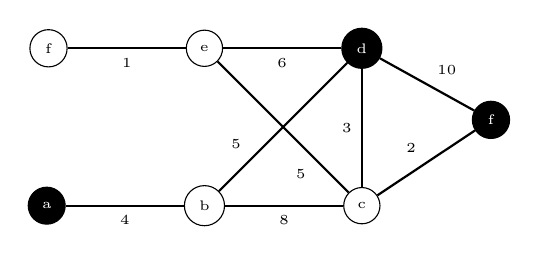
\begin{tikzpicture}[auto, node distance=1.5 cm]
  %Nodes
  \node[terminal] (a) {a};
  \node[steiner] (b) [right=of a] {b};
  \node[steiner] (c) [right=of b] {c};
  \node[terminal] (d) [above =of c] {d};
  \node[steiner] (e) [left=of d] {e};
  \node[steiner] (f) [left=of e] {f};
  \node[terminal] (g) [above right=0.75 and 1.3 of c] {f};
  % Edges
  \begin{scope}[every edge/.style={draw=black, thick}]
    \draw (a) edge node[below]{4} (b);
    \draw (b) edge node[near start]{5} (d);
    \draw (b) edge node[below]{8} (c);
    \draw (c) edge node{3} (d);
    \draw (c) edge node{2} (g);
    \draw (c) edge node[near start]{5} (e);
    \draw (d) edge node{6} (e);
    \draw (d) edge node{10} (g);
    \draw (e) edge node{1} (f);
  \end{scope}
\end{tikzpicture}
\caption{Instance of the Steiner Tree Problem. Terminals are coloured black and non-terminals coloured white.}
\label{fig:stp:01}
\end{figure}

Figure (\ref{fig:stp:01}) shows an instance of the STP with three terminals and four Steiner points. Since vertices
A, C, and D are terminals, they must be spanned by any feasible solution. Figure (\ref{fig:stp:01:feasible}) shows
a feasible solution (which we here denote as a set of edges)
$$E_T = \{(a,b), (b,d), (d,g)\}$$
with cost
$$c(T) = 4 + 5 + 10 = 19\mathnormal{.}$$
However, $T$ is not a Steiner tree as there exists at least one feasible solution with lower cost, i.e. the solution
$$E_{T'} = \{(a,b), (b,d), (d,c), (c,g)\}$$
in Figure (\ref{fig:stp:01:min}) which has cost
$$c(T') = 4 + 5 + 3 + 2 = 14\mathnormal{.}$$
% Suboptimal and Optimal STP solutions 
\begin{figure}[h]\centering
  \begin{subfigure}{0.47\linewidth}
    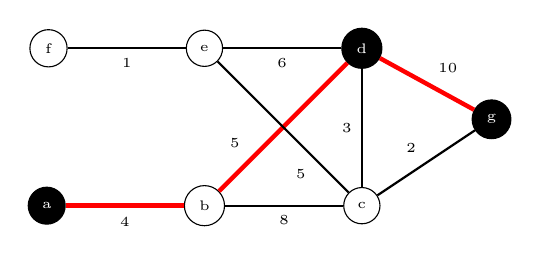
\begin{tikzpicture}[auto, node distance=1.5 cm]
      % Nodes
      \node[terminal] (a) {a};
      \node[steiner] (b) [right=of a] {b};
      \node[steiner] (c) [right=of b] {c};
      \node[terminal] (d) [above =of c] {d};
      \node[steiner] (e) [left=of d] {e};
      \node[steiner] (f) [left=of e] {f};
      \node[terminal] (g) [above right=0.75 and 1.3 of c] {g};
      % Edges
      \begin{scope}[every edge/.style={draw=black, thick}]
        \draw (a) edge[selected] node[below]{4} (b);
        \draw (b) edge[selected] node[near start]{5} (d);
        \draw (b) edge node[below]{8} (c);
        \draw (c) edge node{3} (d);
        \draw (c) edge node{2} (g);
        \draw (c) edge node[near start]{5} (e);
        \draw (d) edge node{6} (e);
        \draw (d) edge[selected] node{10} (g);
        \draw (e) edge node{1} (f);
      \end{scope}
    \end{tikzpicture}
    \caption{Feasible but not optimal.}
    \label{fig:stp:01:feasible}
  \end{subfigure}
  \quad
  \begin{subfigure}{0.47\linewidth}
    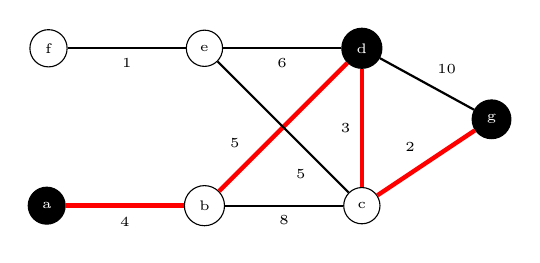
\begin{tikzpicture}[auto, node distance=1.5 cm]
      % Nodes
      \node[terminal] (a) {a};
      \node[steiner] (b) [right=of a] {b};
      \node[steiner] (c) [right=of b] {c};
      \node[terminal] (d) [above =of c] {d};
      \node[steiner] (e) [left=of d] {e};
      \node[steiner] (f) [left=of e] {f};
      \node[terminal] (g) [above right=0.75 and 1.3 of c] {g};
      % Edges
      \begin{scope}[every edge/.style={draw=black, thick}]
        \draw (a) edge[selected] node[below]{4} (b);
        \draw (b) edge node[below]{8} (c);
        \draw (b) edge[selected] node[near start]{5} (d);
        \draw (c) edge[selected] node{3} (d);
        \draw (c) edge[selected] node{2} (g);
        \draw (c) edge node[near start]{5} (e);
        \draw (d) edge node{6} (e);
        \draw (d) edge node{10} (g);
        \draw (e) edge node{1} (f);
      \end{scope}
    \end{tikzpicture}

    \caption{Minimal weight, optimal.}
    \label{fig:stp:01:min}
  \end{subfigure}
  \caption{Solutions to the STP in (\ref{fig:stp:01}). Red edges are part of the solution.}
\end{figure} 

\subsection{ILP Formulations}

\paragraph{Cut Formulation} Let $x$ be a decision vector of length $|E|$ where
$x_{ij} = 1$ implies that $(i,j) \in T$ and $x_{ij} = 0$ implies that $(i,j) \not\in T$,
 and let $c$ be a vector of node-weight s.t. $c_{ij} = c((i,j))$.
Then define the function $x : E \to \ZZ$ as
$$x(E') = \sum_{i,j \in E'} x_{ij}$$
that is, $x(E)$ is equal to the number of selected edges in $E$.
Finally let,
$$\delta(S) = \{(i, j) \mid i \in S \wedge j \in (E \setminus S)\}$$
be all edges which span the cut defined by $S$. Then we can formulate
 the STP as in ILP in terms of cuts (see Formulation (\ref{form:stp:cut})).
 \begin{formulation}[h!]
   \begin{subequations}
     \begin{alignat}{3} %TODO: Find reference for this formulation
       &\underset{x}{\text{minimize}}
       & & c^T x & \\
       & \text{subject to}\quad
       & & x(\delta(S)) \geq 1 \qquad&& \forall S \subset V \label{form:stp:cut:cut}\\
       &&&&& S \cap N \neq \emptyset \nonumber\\
       &&&&& S \cap (V \setminus N) \neq \emptyset \nonumber\\
       &&& x \in \BB. &&
     \end{alignat}\label{form:stp:cut}
   \end{subequations}
   \caption{The \textit{Cut Formulation} of the STP \citep{koch1998solving}.}
 \end{formulation}

 Constraints (\ref{form:stp:cut:cut}) ensures that any feasible solution, $T$,  must span all terminals in $G$, by
 requiring that every Steiner cut in $G$ must be crossed by an edge in $T$. This, combined with objective function
  ensures that any optimal solution to (\ref{form:stp:cut}) must be a Steiner tree in $G$ and vice versa.

\section{Steiner Aborescence Problem}
The Steiner Aborescence Problem (SAP) is the directed version of the Steiner Tree Problem.
Given a \textit{directed} graph,
$$G = (V, A, c)$$
a non-empty terminal set $N \subseteq V$, a root terminal $r \in N$, and arc-weights $c : A \to \RR^+$,
then a Steiner Aborescence, $T \subseteq A$, is an aborescence
in $G$, rooted in $r$, which spans $N$ and has minimal cost.

As with the STP, we denote vertices in $N$ as \textit{terminals}, and any non-terminals spanned by a Steiner Aborescence as
 \textit{Steiner vertices} or \textit{Steiner Points}.
\begin{figure}[h]\centering
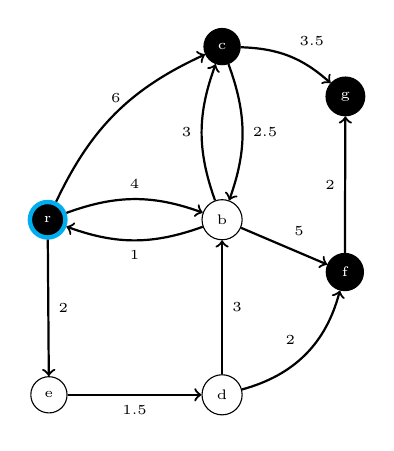
\begin{tikzpicture}[auto, node distance=1.7 cm]
  %Nodes
  \node[terminal, root] (r) at (0,0) {r};
  \node[steiner] (b) [right= of r] {b};
  \node[terminal] (c) [above= of b] {c};
  \node[steiner] (d) [below= of b] {d};
  \node[steiner] (e) [left= of d] {e};
  \node[terminal] (f) [above right= of d] {f};
  \node[terminal] (g) [above right= of b] {g};
  % Edges
  \begin{scope}[every edge/.style={draw=black, thick}]
    \draw[->] (r) edge [bend left=20] node[above]{4} (b);
    \draw[<-] (r) edge [bend right=20] node[below]{1} (b);
    \draw[->] (r) edge [bend left=20] node[above]{6} (c);
    \draw[->] (r) edge  node{2} (e);
    \draw[->] (b) edge [bend left=20] node{3} (c);
    \draw[<-] (b) edge [bend right=20] node[swap]{2.5} (c);
    \draw[<-] (b) edge  node{3} (d);
    \draw[->] (b) edge  node{5} (f);
    \draw[->] (c) edge [bend left=20] node{3.5} (g);
    \draw[<-] (d) edge  node{1.5} (e);
    \draw[->] (d) edge [bend right] node{2} (f);
    \draw[->] (f) edge node{2} (g);
  \end{scope}
\end{tikzpicture}
\caption{Instance of the Steiner Aborescence Problem. Terminals are coloured black, non-terminals are coloured white, and the root terminal
  has a blue outline.}
\label{fig:sap:01}
\end{figure}

Figure (\ref{fig:sap:01}) shows an instance of the SAP with four terminals. Figure (\ref{fig:sap:01:opt}) shows a Steiner Aborescence in (\ref{fig:sap:01})
with cost $c(T) = 13.5$. It is worth noting that since all arcs must point away from the root in an aborescence, while the path $c, b, r$  has
 lower cost than the arc $(r, c)$, it cannot be part of a solution. Similarly, solutions to the SAP in the same graph but with root $c$ have lower cost.

\begin{figure}[h]\centering
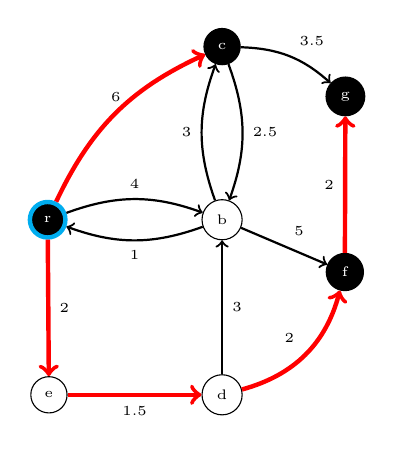
\begin{tikzpicture}[auto, node distance=1.7 cm]
  %Nodes
  \node[terminal, root] (r) at (0,0) {r};
  \node[steiner] (b) [right= of r] {b};
  \node[terminal] (c) [above= of b] {c};
  \node[steiner] (d) [below= of b] {d};
  \node[steiner] (e) [left= of d] {e};
  \node[terminal] (f) [above right= of d] {f};
  \node[terminal] (g) [above right= of b] {g};
  % Edges
  \begin{scope}[every edge/.style={draw=black, thick}]
    \draw[->] (r) edge [bend left=20] node[above]{4} (b);
    \draw[<-] (r) edge [bend right=20] node[below]{1} (b);
    \draw[->] (r) edge [bend left=20, selected] node[above]{6} (c);
    \draw[->] (r) edge [selected] node{2} (e);
    \draw[->] (b) edge [bend left=20] node{3} (c);
    \draw[<-] (b) edge [bend right=20] node[swap]{2.5} (c);
    \draw[<-] (b) edge  node{3} (d);
    \draw[->] (b) edge  node{5} (f);
    \draw[->] (c) edge [bend left=20] node{3.5} (g);
    \draw[<-] (d) edge [selected, selected] node{1.5} (e);
    \draw[->] (d) edge [bend right, selected] node{2} (f);
    \draw[->] (f) edge [selected] node{2} (g);
  \end{scope}
\end{tikzpicture}
\caption{Steiner Aborescence in (\ref{fig:sap:01}) with cost $13.5$.}
\label{fig:sap:01:opt}
\end{figure}

The SAP is relevant mainly due to a tendency of reformulating the undirected STP into the SAP \citep{koch1998solving}, as well as reformulating
the PCSTP into the SAP \citep{gamrath2017scip, Ljubic:2004:memetic} and
prize-collecting variants of the SAP \citep{leitner2016dual, ljubic2005solving} before stating them as integer programs. This is due to results which show that LP relaxations of
 directed Steiner Tree Problem variants behave better than undirected variants \citep{Chopra:1994}.

\subsection{Reduction from Other Variants}

\subsubsection{Steiner Tree Problem}
\begin{figure}[h]\centering
  \begin{subfigure}{0.47\linewidth}
    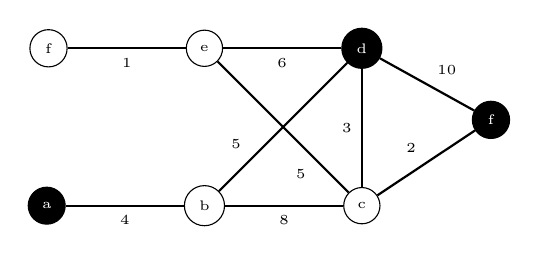
\begin{tikzpicture}[auto, node distance=1.5 cm]
      % Nodes
      \node[terminal] (a) {a};
      \node[steiner] (b) [right=of a] {b};
      \node[steiner] (c) [right=of b] {c};
      \node[terminal] (d) [above =of c] {d};
      \node[steiner] (e) [left=of d] {e};
      \node[steiner] (f) [left=of e] {f};
      \node[terminal] (g) [above right=0.75 and 1.3 of c] {f};
      % Edges
      \begin{scope}[every edge/.style={draw=black, thick}]
        \draw (a) edge node[below]{4} (b);
        \draw (b) edge node[near start]{5} (d);
        \draw (b) edge node[below]{8} (c);
        \draw (c) edge node{3} (d);
        \draw (c) edge node{2} (g);
        \draw (c) edge node[near start]{5} (e);
        \draw (d) edge node{6} (e);
        \draw (d) edge node{10} (g);
        \draw (e) edge node{1} (f);
      \end{scope}
    \end{tikzpicture}
    \caption{Problem Instance (\ref{fig:stp:01})}
  \end{subfigure}
  \begin{subfigure}{0.47\linewidth}
    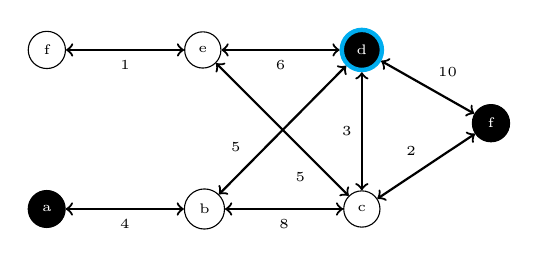
\begin{tikzpicture}[auto, node distance=1.5 cm]
      % Nodes
      \node[terminal] (a) {a};
      \node[steiner] (b) [right=of a] {b};
      \node[steiner] (c) [right=of b] {c};
      \node[terminal, root] (d) [above =of c] {d};
      \node[steiner] (e) [left=of d] {e};
      \node[steiner] (f) [left=of e] {f};
      \node[terminal] (g) [above right=0.75 and 1.3 of c] {f};
      % Edges
      \begin{scope}[every edge/.style={draw=black, thick}]
        \draw[<->] (a) edge node[below]{4} (b);
        \draw[<->] (b) edge node[near start]{5} (d);
        \draw[<->] (b) edge node[below]{8} (c);
        \draw[<->] (c) edge node{3} (d);
        \draw[<->] (c) edge node{2} (g);
        \draw[<->] (c) edge node[near start]{5} (e);
        \draw[<->] (d) edge node{6} (e);
        \draw[<->] (d) edge node{10} (g);
        \draw[<->] (e) edge node{1} (f);
      \end{scope}
    \end{tikzpicture}
    \caption{Instance (\ref{fig:stp:01}) as a SAP instance. Root node is coloured blue.}
  \end{subfigure}
  \caption{Reduction from STP to SAP.}
  \label{fig:stptosap}
\end{figure}

\subsubsection{Prize-Collecting Steiner Tree Problem}

\subsection{ILP Formulations}
\section{Prize-Collecting Steiner Tree Problem}
Given an undirected graph
$$G = (V, E, c, p)$$
where $c: E \to \RR^+$ defines edge weights,
and $p: V \to \RR^+$ defines vertex \textit{prizes}, then the solution to the \textit{Prize-Collecting
  Steiner Tree Problem} (PCSTP) is a tree
$$T = (V_T, E_T, c, p) \subseteq G$$
which minimizes
$$GW(T) = \sum_{(i,j) \in E_T} c_{ij} + \sum_{v\in (V_T \setminus V)} p_v$$
which is also known as the {\textit{Goemans-Williamson Minimization Problem}}.

The PCSTP can equilvalently be stated as the {\textit{Net Worth Maximization Problem}} \citep{Johnson:2000:PCS:338219.338637},
$$NW(T) = \sum_{v \in V_T} p_v - \sum_{(i,j) \in E_T} c_{ij} \mathnormal{.}$$
In the context of the PCSTP, We denote vertices with nonzero prize as \textit{terminals}, giving the terminal set
$$N = \{v \mid p_v > 0\} \subseteq V\mathnormal{.}$$

\begin{figure}[h]\centering
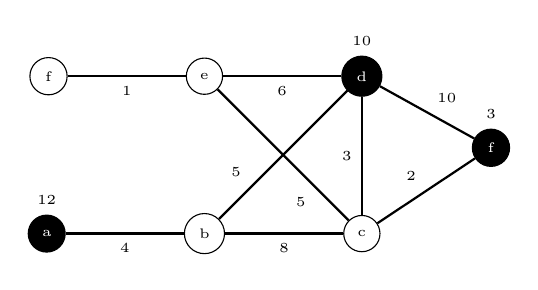
\begin{tikzpicture}[auto, node distance=1.5 cm]
  %Nodes
  \node[terminal, label={12}] (a) {a};
  \node[steiner] (b) [right=of a] {b};
  \node[steiner] (c) [right=of b] {c};
  \node[terminal, label={10}] (d) [above =of c] {d};
  \node[steiner] (e) [left=of d] {e};
  \node[steiner] (f) [left=of e] {f};
  \node[terminal, label={3}] (g) [above right=0.75 and 1.3 of c] {f};
  % Edges
  \begin{scope}[every edge/.style={draw=black, thick}]
    \draw (a) edge node[below]{4} (b);
    \draw (b) edge node[near start]{5} (d);
    \draw (b) edge node[below]{8} (c);
    \draw (c) edge node{3} (d);
    \draw (c) edge node{2} (g);
    \draw (c) edge node[near start]{5} (e);
    \draw (d) edge node{6} (e);
    \draw (d) edge node{10} (g);
    \draw (e) edge node{1} (f);
  \end{scope}
\end{tikzpicture}
\caption{Instance of the Prize-Collecting Steiner Tree Problem. Terminals are coloured black and non-terminals coloured white.}
\label{fig:pcstp:01}
\end{figure}

Figure (\ref{fig:pcstp:01}) shows an instance, $G$, of the PCSTP created by assigning prizes to the terminals of the STP instance, $G_{STP}$, in Figure (\ref{fig:stp:01}).
Figure (\ref{fig:pcstp:01})
shows an optimal solution, $T = (V_T, E_T)$, to $G$. An interesting observation is that
$T$ is a sub-graph of the solution in Figure (\ref{fig:stp:01:min}) to $G_{STP}$.
In fact, if we were to modify $G_{STP}$ by setting its terminal set to the vertices spanned
by $T$, that is we define $G'_{STP} =  G_{STP}$ where  $N_{G'_{STP}} = V_T$, then $T$ is a Steiner
tree in $G'_{STP}$. In other words, we can describe the search space of the PCSTP
 as the set of all Steiner trees in a graph $G$.

\begin{figure}[h]\centering
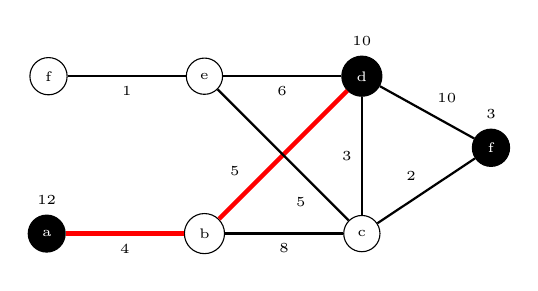
\begin{tikzpicture}[auto, node distance=1.5 cm]
  %Nodes
  \node[terminal, label={12}] (a) {a};
  \node[steiner] (b) [right=of a] {b};
  \node[steiner] (c) [right=of b] {c};
  \node[terminal, label={10}] (d) [above =of c] {d};
  \node[steiner] (e) [left=of d] {e};
  \node[steiner] (f) [left=of e] {f};
  \node[terminal, label={3}] (g) [above right=0.75 and 1.3 of c] {f};
  % Edges
  \begin{scope}[every edge/.style={draw=black, thick}]
    \draw (a) edge[selected] node[below]{4} (b);
    \draw (b) edge[selected] node[near start]{5} (d);
    \draw (b) edge node[below]{8} (c);
    \draw (c) edge node{3} (d);
    \draw (c) edge node{2} (g);
    \draw (c) edge node[near start]{5} (e);
    \draw (d) edge node{6} (e);
    \draw (d) edge node{10} (g);
    \draw (e) edge node{1} (f);
  \end{scope}
\end{tikzpicture}
\caption{Optimal solution to (\ref{fig:pcstp:01})\textnormal{.}}
\label{fig:pcstp:01:opt}
\end{figure}

Unsurprisingly, the PCSTP is an NP-Hard problem. It is a generalisation of the STP. Any instance of
the STP with graph $G = (V, E, c)$ and terminal set $N$ can be reduced to an instance of the PCSTP
with graph $G' = (V, E, c, p)$ where
where
$$p_v =
\begin{cases}
  \infty & v \in N\mathnormal{,} \\
  0 & \mathnormal{otherwise.}
\end{cases}$$
Any optimal solution to $G'$ is then a Steiner tree in $G$ and vice versa.
\subsection{ILP Formulations}
%%% Local Variables:
%%% TeX-master: "report"
%%% reftex-default-bibliography: ("lit.bib")
%%% End:

\chapter{Solving the Prize-Collecting Steiner Tree Problem}
\label{chap:solving}
\section{Preprocessing}
Applying preprocessing routines to heavily reduce input graphs is a common technique which has been proven succesful in many cases both for instances of the STP
\citep{koch1998solving}
and instances of the PCSTP
\citep{ljubic2005solving, gamrath2017scip}. %TODO: MORE
These routines make use of proven invariants to remove and contract edges as well as choose edges before applying the any main procedure.
A set of common preprocessing routines are applied in different manners in literature, mainly differentiated by:
\begin{enumerate}[label=\alph*)]
\item which routines to apply,
\item in which order, and
\item when to recursively apply routines and how many times.
\end{enumerate}
Preprocessing routines can be very effective. For example, the preprocesing routine presented by \cite{koch1998solving} for the STP removes
up to 98\% of edges in some instances. In this section, we will first give a full overview of existing preprocessing methods for the PCSTP,
 including proofs of validity,
 and then summarize their usage in recent literature.

 In the following, we will denote any edge or vertex (or part of a graph) as \textit{redundant} if there exists an optimal solution
  which does not contain it, and we say that a 
  transformation to a problem instance is \textit{valid} when produces an equivalent problem, that is a problem which has the same optimal
  value and in which solutions map back to the original problem.

 \subsection{Local Reduction Tests}
 The first type of reductions we will look at, we will named \textit{local} reduction tests. These are tests which only require knowledge
 of the neighbourhood of a couple of vertexes in the graph, and perhaps simple global information such as maximum prize. As such, the tests
 presented in this section are generally of low computational cost, allowing for testing a full graph in linear time.

 Note that the first tests presented (NTD1, NTD2, TD1, TD2) are known collectively
 in recent literature as \textit{Degree Tests}, for example in \cite{rehfeldt2016reduction}.
\subsubsection{Non-Terminals of Degree 1}
\label{sec:red:test:deg1}
Let $G = (V, E, c, p)$ be a PCST instance and let $v \in V$ be any non-terminal with degree 1, then
 clearly -- since edges have positive weights -- $v$ can not be part of an optimal solution. Thus $v$ is redundant. In other words,
 all vertices in the set
 $$\{v \mid v \in V \setminus N \wedge |\delta(v)| = 1\}$$
 are redundant and it is valid to remove them from $G$ along with their adjacent edges.

\begin{figure}[h]\centering
    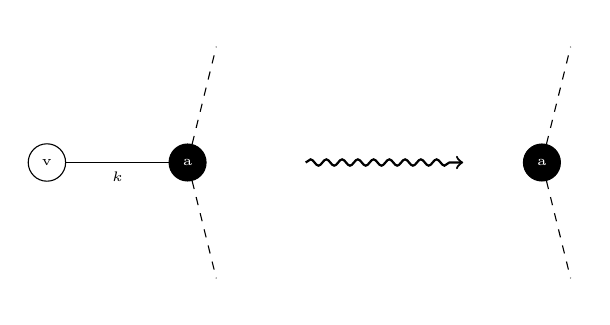
\begin{tikzpicture}[auto, node distance=1.3 cm]
      % Pre
      \begin{scope}[shift={(-0.5,0)}]
        \node[terminal] (a) at (0, 0) {a};
        \node[steiner] (b) [left=of a] {v};
        \node (sg) [above right = 1.3 and 0.1 of a] {};
        \node (sg2) [below right= 1.3 and 0.1 of a] {};

        %Edges
        \draw (a) edge node {$k$} (b);
        \draw[dashed] (a) to (sg);
        \draw[dashed] (a) to (sg2);
      \end{scope}

      \draw [->,decorate, thick,
      decoration={snake,amplitude=.4mm,segment length=2mm,post length=1mm}]
      (1.0,0) -- (3,0);
      % Post      
      \begin{scope}[shift={(4cm, 0)}]

        \node[terminal] (a) at (0, 0) {a};
        \node (sg) [above right = 1.3 and 0.1 of a] {};
        \node (sg2) [below right= 1.3 and 0.1 of a] {};

        %Edges
        \draw[dashed] (a) to (sg);
        \draw[dashed] (a) to (sg2);
      \end{scope}

  \end{tikzpicture}
  \caption{Removing a non-terminal with degree 1.}
  \label{fig:red:test:deg1}
\end{figure}

 While this reduction test is originally stated for the STP \citep{hwang1992steiner}, it is also applicable to the PCSTP. Figure (\ref{fig:red:test:deg1})
  shows an example of removing a degree 1 non-terminal.

  \subsubsection{Non-Terminals of Degree 2}
    \label{fig:red:test2}
\todo{These two sections probably use too different methods in defining their reductions}
    Similarly, let $G = (V,E,c,p)$ be an instance of the PCSTP, let $v \in G$ be a non-terminal with degree $|\delta(v)| = 2$, and let
    $u$ and $w$ be the two vertices adjacent to $v$. Then we can obtain a reduced, equivalent graph,
    $$G' = (V', E', c', p)$$
    where
    $$V' = V - v \mathnormal{,}$$
    $$E' = (E \setminus \{(u,v),(w,v)\}) \cup \{(u,w)\}\mathnormal{,}$$
    and
    $$c_{uw} =
    \begin{cases}
      \min(c_{uw}, c_{uv} + c_{vw}) & (u,w) \in E\mathnormal{,} \\
      c_{uv} + c_{vw} & \text{otherwise.}
    \end{cases}$$

    In other words, if $c_{uv} + c_{vw} <  c_{uw}$ then $(u,w)$ is redundant, can be removed, and $v$ and its edges
    can be contracted to a single edge.
    Otherwise $v$ and its edges are redundant and can be removed. Figure (\ref{fig:red:test:deg2})
    shows an example this reduction test.

\begin{figure}[h!]\centering
    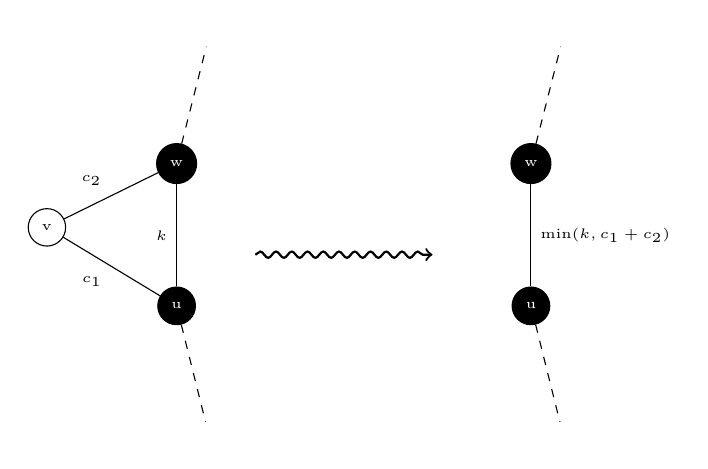
\begin{tikzpicture}[auto, node distance=1.3 cm]
      % Pre
      \begin{scope}
        \node[terminal] (a) at (0, -0.65) {u};
        \node[terminal] (b) [above=of a] {w};
        \node[steiner] (c) [above left= 0.65 and 1.3 of a] {v};
        \node (sg) [above right = 1.3 and 0.1 of b] {};
        \node (sg2) [below right= 1.3 and 0.1 of a] {};

        %Edges
        \draw (a) edge node {$k$} (b);
        \draw (a) edge node {$c_1$} (c);
        \draw (b) edge node[swap] {$c_2$} (c);
        \draw[dashed] (b) to (sg);
        \draw[dashed] (a) to (sg2);
      \end{scope}

      \draw [->,decorate, thick,
      decoration={snake,amplitude=.4mm,segment length=2mm,post length=1mm}]
      (1,0) -- (3.25,0);
      % Post      
      \begin{scope}[shift={(4.5cm, 0)}]
        \node[terminal] (a) at (0, -0.65) {u};
        \node[terminal] (b) [above=of a] {w};
        \node (sg) [above right = 1.3 and 0.1 of b] {};
        \node (sg2) [below right= 1.3 and 0.1 of a] {};

        %Edges
        \draw (a) edge node[swap] {$\min(k, c_1 + c_2)$} (b);
        \draw[dashed] (b) to (sg);
        \draw[dashed] (a) to (sg2);
      \end{scope}

  \end{tikzpicture}
  \caption{Removing a non-terminal with degree 2.}
  \label{fig:red:test:deg2}
\end{figure}

This test is another example of a reduction test for the STP which can by directly applied to
 the PCSTP.
\subsubsection{Terminals of Degree 1}
\label{sec:red:test:tdeg1}
\todo[inline]{Write this section. It's very clear.}
\begin{figure}[h!]\centering
    \begin{tikzpicture}[auto, node distance=1.3 cm]
      % Pre
      \begin{scope}[shift={(-0.5,0)}]
        \node[terminal, label={$p_a$}] (a) at (0, 0) {a};
        \node[terminal, label={$p_v$}] (b) [left=of a] {v};
        \node (sg) [above right = 1.3 and 0.1 of a] {};
        \node (sg2) [below right= 1.3 and 0.1 of a] {};

        %Edges
        \draw (a) edge node {$k$} (b);
        \draw[dashed] (a) to (sg);
        \draw[dashed] (a) to (sg2);
      \end{scope}

      \draw [->,decorate, thick,
      decoration={snake,amplitude=.4mm,segment length=2mm,post length=1mm}]
      (1.0,1) -- node [above=1mm,midway,text width=3cm, sloped, align=center] {$k\geq p_v$}
      (3,2);
      % Post      
      \begin{scope}[shift={(6cm, 3cm)}]

        \node[terminal, label=right:{$p_a$}] (a) at (0, 0) {a};
        \node[terminal, label={$p_v$}] (b) [left=of a] {v};
        
        \node (sg) [above right = 1.3 and 0.1 of a] {};
        \node (sg2) [below right= 1.3 and 0.1 of a] {};

        %Edges
        \draw[dashed] (a) to (sg);
        \draw[dashed] (a) to (sg2);
      \end{scope}

      \draw [->,decorate, thick,
      decoration={snake,amplitude=.4mm,segment length=2mm,post length=1mm}]
      (1.0,-1) -- node [above=1mm,midway,text width=3cm, sloped, align=center] {$k < p_v$}
      (3,-2);

      % Post2      
      \begin{scope}[shift={(6cm, -3cm)}]
        \node[terminal, label=right:{$p_a + (p_v - k)$}] (a) at (0, 0) {a};
        \node[terminal, label={$p_v$}] (b) [left=of a] {v};

        \node (sg) [above right = 1.3 and 0.1 of a] {};
        \node (sg2) [below right= 1.3 and 0.1 of a] {};

        %Edges
        \draw[dashed] (a) to (sg);
        \draw[dashed] (a) to (sg2);
      \end{scope}

  \end{tikzpicture}
  \caption{Removing the edge connected a terminal of degree 1.}
  \label{fig:red:test:deg1}
\end{figure}

\subsubsection{Terminals of Degree 2}


\subsubsection{Minimum Adjacency}
Again defined in \cite{duin1989reduction} for the STP, the \textit{minimum adjacency test}
(also known as the \textit{$V \setminus K$ test}) is a reduction test which contracts adjacent
terminals as shown in Figure (\ref{fig:red:test:ma}).
 
\begin{figure}[h!]\centering
    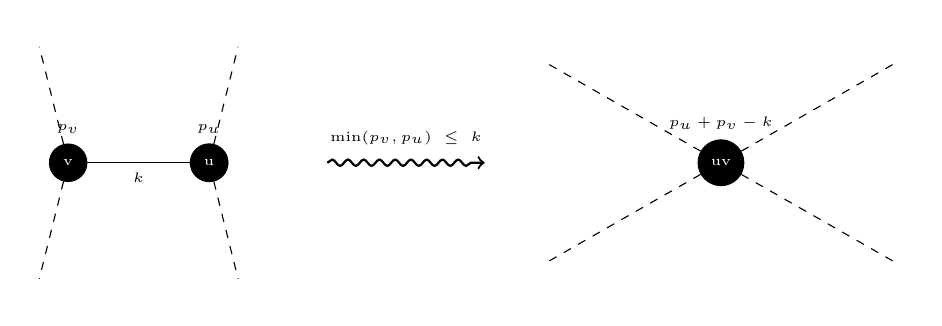
\begin{tikzpicture}[auto, node distance=1.3 cm]
      % Pre
      \begin{scope}[shift={(-0.5,0)}]
        \node[terminal, label={$p_u$}] (u) at (0, 0) {u};
        \node[terminal, label={$p_v$}] (v) [left=of u] {v};
        \node (sgu) [above right = 1.3 and 0.1 of u] {};
        \node (sgu2) [below right= 1.3 and 0.1 of u] {};

        \node (sgv) [above left = 1.3 and 0.1 of v] {};
        \node (sgv2) [below left= 1.3 and 0.1 of v] {};

        %Edges
        \draw (u) edge node {$k$} (v);
        \draw[dashed] (u) to (sgu);
        \draw[dashed] (u) to (sgu2);
        \draw[dashed] (v) to (sgv);
        \draw[dashed] (v) to (sgv2);
      \end{scope}

      \draw [->,decorate, thick,
      decoration={snake,amplitude=.4mm,segment length=2mm,post length=1mm}]
      (1.0,0) -- node [above=1mm,midway,text width=3cm, sloped, align=center] {$\min(p_v, p_u) \leq k$}
      (3,0);
      % Post      
      \begin{scope}[shift={(6cm, 0cm)}]
        \node[terminal, label={$p_u + p_v - k$}] (u) at (0, 0) {uv};
        \node (sgu) [above right = 1. and 2.0 of u] {};
        \node (sgu2) [below right= 1. and 2.0 of u] {};
        \node (sgv) [above left = 1. and 2.0 of u] {};
        \node (sgv2) [below left= 1. and 2.0 of u] {};

        %Edges
        \draw[dashed] (u) to (sgu);
        \draw[dashed] (u) to (sgu2);
        \draw[dashed] (u) to (sgv);
        \draw[dashed] (u) to (sgv2);
      \end{scope}

  \end{tikzpicture}
  \caption{Minimum adjacency test.}
  \label{fig:red:test:ma}
\end{figure}

\begin{theorem}[Minimum Adjacency]
  Let $u$ and $v$ be adjacent terminals in $G$. If we have
  $$\min(p_u, p_v) \geq c_{uv}$$
  and
  $$c_{uv} = \min_{(u, w) \in E}c_{uw}$$
  then it is valid to contract $u$ and $v$.
\end{theorem}
\begin{proof}
  It can be shown that any solution $T$ for the PCSTP problem defined by a graph $G$
  which contains $u$ but not $(u,v)$ can
  be transformed into a solution $T'$ which contains $(u,v)$ where $c(T') \leq c(T)$.

  \paragraph{Case 1: $v \in V_T$}
  Let $(u, w) \in E_T$ be the first edge in the simple path from $u$ to $v$. By assumption, we
  have that $c_{uv} \leq c_{uw}$, and the tree $T'$ constructed by removing $(u,w)$ from $T$ and
  adding $(u,v)$ has cost
  $$c(T') = c(T) - c_{uw} + c_{uv} \leq T\mathnormal{.}$$
  \paragraph{Case 2: $v  \not\in V_T$}
  Let $T'$ be the tree obtained by adding $(u,v)$ to $T$. As per the assumption that $\min(p_u, p_v) \geq c_{uv}$,
  we have that $T'$ has cost,
  $$c(T') = c(T) + c_{uv} - p_{uv} \leq c(T)\mathnormal{.}$$
\end{proof}

\subsubsection{Unconnected Dominated Vertex}


\subsection{Steiner Distance Reduction Tests}
% $$d(u,v) = \min \{ c(P) \mid P \in \mathcal{P}_{uv}\}$$
More complex tests can be described in terms
of the concepts Steiner distance and Bottleneck distance. These were originally stated for
the STP in, amongst others, \cite{duin1989edge,duin1989reduction} and later
adapted for the PCSTP in \cite{uchoa2006reduction}.

First we must make some definitions.
If $P = (..., u, ..., w, ...)$ is a simple path in $G$, then $P_{uw}$ is
the subpath in $P$ starting at vertex $u$ and ending in vertex $w$,
\todo{Some of this should probably go in a notations section}
that is $P_{u,w} = (u, ...,w)$. Then we define the \textit{Steiner distance} of
 $P_{uw}$ as,

 $$sd(P_{uw}) = \sum_{(i,j) \in E(P_{u,w})} c_{i,j} -
 \sum_{v \in V(P) \setminus \{u,w\}} p_{v}\mathnormal{.}$$
 We then denote the Steiner distance of a simple path, $P$, as the maximal Steiner
 distance found among subpaths of $P$,
 $$sd(P) = \max_{u,w \in P} sd(P_{uw})\mathnormal{.}$$
 Let $\mathcal{P}_{uw}$ be the set of all simple paths
 connecting vertices $u$ and $w$ in
 $G$, then we denote the \textit{bottleneck distance} between $u$ and $w$ as minimal Steiner
  distance among paths in $\mathcal{P}_{uw}$,
  $$B(u,w) = \min_{P \in  \mathcal{P}_{uw}} sd(P)\mathnormal{.}$$
  The bottleneck distance is a measure of the worst case \textit{additional cost}
  \todo{Make decision on whether I should replicated proofs for claims like this.}
 of connecting
 two disjoint subgraphs containing vertices $u$ and $v$ respectively in $G$.

  \missingfigure{Some visual intuition on the bottleneck distance}

  Finally, we denote the bottleneck distance between vertices $u$ and $w$ \textit{excluding}
  the edge $e$ as,
  $$B(u,w)^{-e} = \min_{P \in  \mathcal{P}_{uw}, e \not \in P} sd(P)\mathnormal{.}$$


 \cite{uchoa2006reduction} shows that calculating the bottleneck distance
 is an NP hard problem by reduction from the Hamiltonian Path problem. Hence,
 exactly calculating the bottleneck distance is infeasible. However, \cite{uchoa2006reduction}
 also claims that existing heuristics are fast and give strong upper bounds.
 \subsubsection{Special Distance}
 \label{sec:red:test:sd}
 Using the PCSTP version of the Steiner and bottleneck distances, \cite{uchoa2006reduction} proves
  the validity of the more general \textit{special distance test}.
 \begin{theorem}[Special Distance Test]
 Consider any edge $(u,v) \in E$. If we have
 $$B(u,v)^{-(u,v)} \leq c_{uv}$$
 then $(u,v)$ is redundant.
\end{theorem}
 \begin{proof}
   Let $T  \subseteq G$ be an optimal solution to the PCSTP in graph $G$
   where we have
   $$B(u,v)^{-(u,v)} \leq c_{uv}$$
   for some edge $(u,v) \in E_T$, and let $(T_1, T_2)$ be the cut bridged
   by $(u,v)$.

   Consider then the simple path $P \in \mathcal{P}_{uv}$ from $u$ to $v$ which doesn't
    contain $(u,v)$ and has
   $$sd(P) = B(u,v)^{-(u,v)}\mathnormal{.}$$

   Since $T$ is a tree, and $P$ by definition doesn't contain the edge $(u,v)$
   then we must have that $P$ consists of a subpath contained in $T_1$, followed by
   a subpath not contained in $T$, followed by a subpath contained in $T_2$.
   In other words, we have,
   $$P = (u, P_1, w, P_2, z, P_3, v)$$
   as shown in Figure \ref{fig:red:test:sd:thm}.

   Then by definition we have,
   $$sd(P_2) \leq sd(P) = B(u,v)^{-(u,v)} \leq c_{uv}$$
   and we construct another solution $T'$ by replacing $(u,v)$ with the
   vertices and edges in $P_2$ which has cost
   $$c(T') = c(T) - c_{uv} + sd(P_2) \leq c(T)\mathnormal{.}$$
   Hence $T'$ also optimal in $G$ and $(u,v)$ is by definition redundant.
\end{proof}
\begin{figure}[h!]\centering
    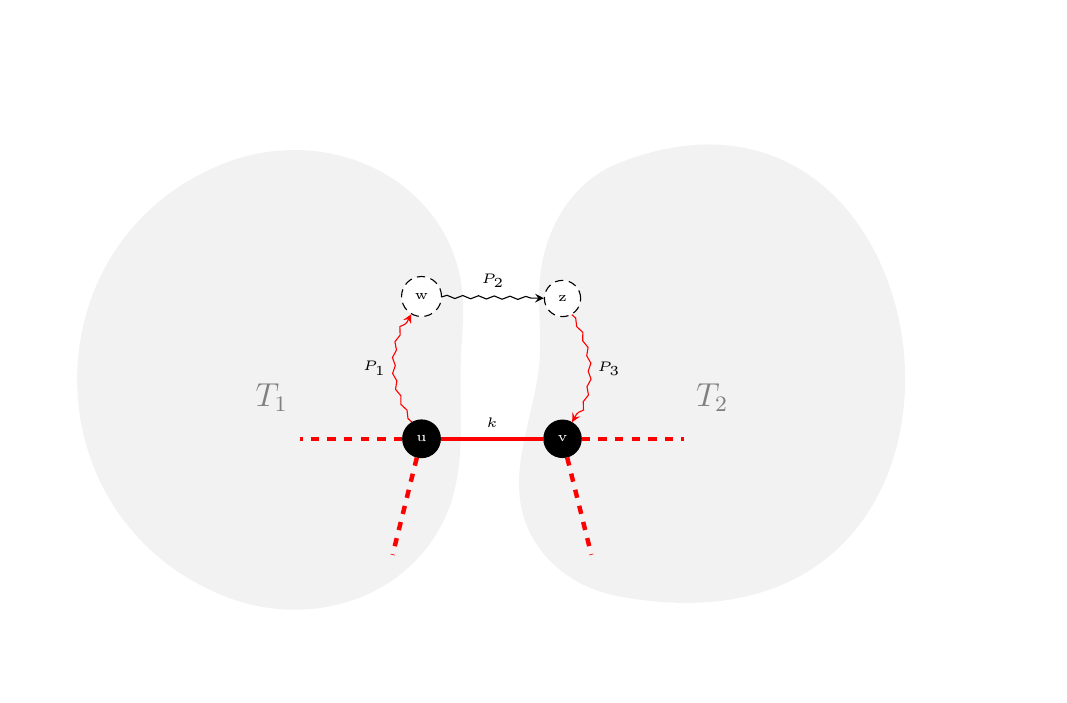
\begin{tikzpicture}[auto, node distance=1.3 cm]
      % Pre
      \begin{scope}[]
        \path[fill=black!5,use Hobby shortcut,closed=true]
        (-2.5, -2) .. (0.3,-1) .. (.5,1) .. (.5,2)  .. (-2.5,3.5);
        \path[fill=black!5,use Hobby shortcut,closed=true]
        (2.5, -2) .. (1.3,-1) .. (1.5,1) .. (1.5,2)  .. (2.5,3.5);

        \node[terminal] (u) at(0, 0) {u};
        \node[subgraph, above left= 0.05cm and 1.4cm of u] {$T_1$};
        \node[steiner, densely dashed] (w1) [above=of u] {w};
        
        \node[terminal] (v) [right= of u] {v};
        \node[subgraph,above right= 0.05 and 1.4cm  of v] {$T_2$};
        \node[steiner, densely dashed] (w2) [above=of v] {z};
        \node (sga) [left= of u] {};
        \node (sga2) [below left= 1.3 and 0.1 of u] {};

        \node (sgb) [right=  of v] {};
        \node (sgb2) [below right= 1.3 and 0.1 of v] {};

        
        
        %Edges
        \draw[selected] (u) edge node {$k$} (v);
        \draw[dashed, selected] (u) to (sga);
        \draw[dashed, selected] (u) to (sga2);

        \draw[dashed, selected] (v) to (sgb);
        \draw[dashed, selected] (v) to (sgb2);

        \draw (u) edge[snake it, red, bend left] node[text=black] {$P_1$} (w1);
        \draw (w1) edge[snake it] node {$P_2$} (w2);
        \draw (w2) edge[snake it, red, bend left] node[text=black] {$P_3$} (v);
      \end{scope}

      % \draw [->,decorate, thick,
      % decoration={snake,amplitude=.4mm,segment length=2mm,post length=1mm}]
      % (4,0) -- node [above=1mm,midway,text width=3cm, sloped, align=center] {}
      % (6,0);
      % Post      

  \end{tikzpicture}
  \caption{The optimal solution, $T = T_1 \cup T_2$ connected by $(u,v)$.
    Since $c(u,v) \geq B(u,v)^{-(u,v)}$,
  the simple path $P_2$ has cost no larger than $(u,v)$ and can replace it in $T$.}
  \label{fig:red:test:sd:thm}
\end{figure}

\subsubsection{Non-Terminals of Degree 3}
\label{sec:red:test:deg3}
Another bottleneck distance based test,
also proved valid for the PCSTP in \cite{uchoa2006reduction},
is the \textit{non-terminals of degree 3 test}.
\begin{theorem}[Non-Terminals of Degree 3 Test]\label{thm:ntd3}
  Let $u$ be a vertex with degree 3 in $G = (V, E, c, p)$,
  and let $v$, $w$, and $z$ be its adjacent
  vertices. If we have
  $$\min\left(B(v,w) + B(v,z), B(w,v) + B(w,z),  B(z, v)+ B(z, w)\right) \leq
  c_{uv} + c_{uw} + c_{uz}$$
  then there exists an optimal solution to $G$ where $u$ has degree of
  \textit{at most} 2, that is $|\delta(u)| \leq 2$. Thus $u$ and its three edges, can be replaced by
  the edges $\{(v, w), (w,z), (z,v)\}$ with costs
  $$c_{vw} = c_{vu} + c_{uw},\quad c_{wz} = c_{wu} + c_{uz},\quad c_{zv} = c_{zu} + c_{uv}\mathnormal{.}$$
\end{theorem}
\begin{proof}   
  W.l.o.g. consider the case where $B(v,w) + B(v,z) \leq c_{uv} + c_{uw} + c_{uz}$,
  and let $T$ be an optimal solution which contains $(u,v)$, $(u,w)$, and $(u,z)$.

  Let $P_1 = (v, ..., w)$ be the simple path with Steiner distance
  $$sd(P_1) = B(v,w)$$
  and similarly let $P_2 = (v, ..., z)$ be the simple path with Steiner distance
  $$sd(P_2) = B(v,z)\mathnormal{.}$$
  This gives us the situation in Figure (\ref{fig:red:test:ntd3:thm}). Note that $u$ may be a part of either paths.

  Let $T_v$, $T_w$, and $T_z$ be the subtrees of $T$ obtained by
  removing the edges adjacent to $u$ from $T$, and construct a new solution with
   total cost no-larger than $T$ as,
   $$T' = T_v \cup T_w \cup T_z \cup P_1 \cup P_2\mathnormal{.}$$
   We must have $|\delta_{T'}(u)| \leq 2$. If we had $|\delta_{T'}| = 3$ then
   we would have
   $$P_1 = \left[v, (v,u), u, (u,w), w \right]$$
   and
   $$P_2 = \left[v, (v,u), u, (u,z) z \right]$$
   giving us
   $$B(v,w) + B(v, z) = sd(P_1) + sd(P_2) = 2 c_{vu} + c_{uw} + c_{uz} > c_{vu} + c_{uw} + c_{uz}$$
   which is a contradiction to our original assumption that
   $$B(v,w) + B(v,z) \leq c_{uv} + c_{uw} + c_{uz}\mathnormal{.}$$
   Thus $T'$ is an optimal solution to $G$ with $|\delta_{T'}(u)| \leq 2$.
\end{proof}
\begin{figure}[h!]\centering
    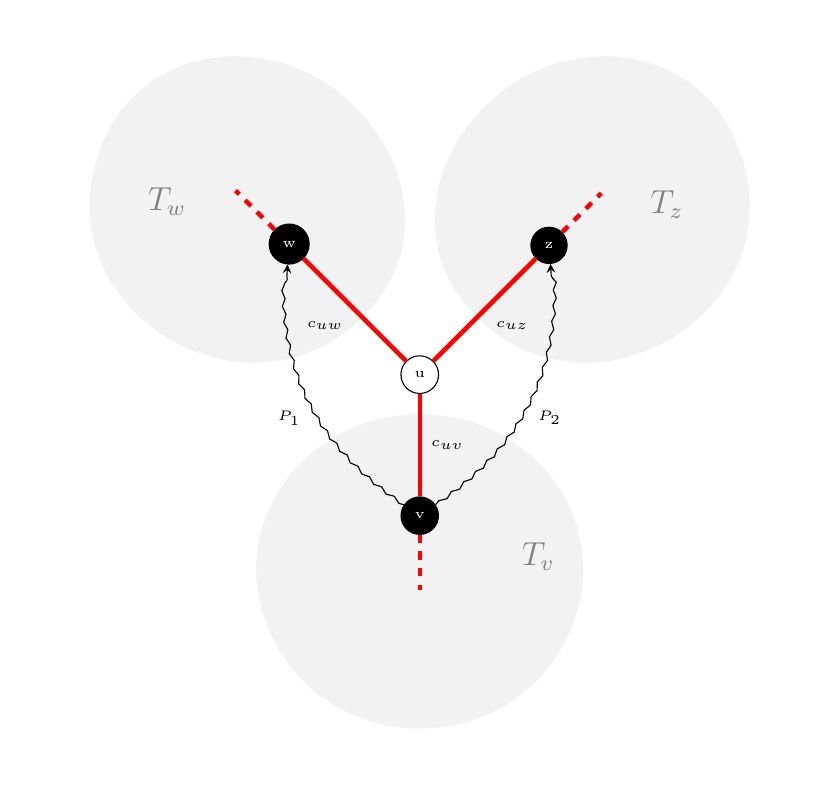
\begin{tikzpicture}[auto, node distance=1.3 cm]
      % Pre
      \begin{scope}[]
        \path[fill=black!5,use Hobby shortcut,closed=true]
        (-0.5, 1) .. (-4, 3) .. (-0.5,3);
        \path[fill=black!5,use Hobby shortcut,closed=true]
        (.5, 1) .. (4,3) .. (.5,3);
        \path[fill=black!5,use Hobby shortcut,closed=true]
        (0, -.5) .. (-2,-3) .. (2,-3);

        \node[steiner] (u) at(0, 0) {u};
        \node[terminal] (w) [above left=1.3 and 1.3 of u] {w};
        \node[terminal] (v) [below= of u] {v};
        \node[terminal] (z) [above right= 1.3 and 1.3 of u] {z};

        \node[subgraph, above left= 0.05cm and 1 cm of w] {$T_w$};
        \node[subgraph,above right= 0.05cm and 1 cm of z] {$T_z$};
        \node[subgraph, below right= 0.05cm and 1 cm of v] {$T_v$};
        
        \node (sgw) [above left= 0.7 of w] {};
        \node (sgv) [below= 0.7 of v] {};
        \node (sgz) [above right = 0.7 of z] {};
        
        %Edges
        \draw[selected] (u) edge node {$c_{uv}$} (v);
        \draw[selected] (u) edge node {$c_{uw}$} (w);
        \draw[selected] (u) edge node[swap] {$c_{uz}$} (z);
        \draw[dashed, selected] (v) to (sgv);
        \draw[dashed, selected] (w) to (sgw);
        \draw[dashed, selected] (z) to (sgz);

        \draw (v) edge[snake it, bend left] node[text=black] {$P_1$} (w);
        \draw (v) edge[snake it, bend right] node[swap,text=black] {$P_2$} (z);
      \end{scope}

      % \draw [->,decorate, thick,
      % decoration={snake,amplitude=.4mm,segment length=2mm,post length=1mm}]
      % (4,0) -- node [above=1mm,midway,text width=3cm, sloped, align=center] {}
      % (6,0);
      % Post      

  \end{tikzpicture}
  \caption{Non-Terminal of $|\delta(u)| = 3$ which connects the subtrees $T_v$, $T_w$, and $T_z$. The simple paths $P_1$ and $P_2$ provide an
     alternate way of reconnecting $T$ with at least as good cost.}
  \label{fig:red:test:ntd3:thm}
\end{figure}

\subsection{Summary of Usage}

\section{Primal Heuristics}

\section{Exact Algorithms}
%%% Local Variables:
%%% TeX-master: "report"
%%% reftex-default-bibliography: ("lit.bib")
%%% End:


\glsresetall
\part{Exploration of Related Problems}
\chapter{Research in Related Problems}
\label{chap:related}
The \gls{pcstp}, while unique in formulation,
is part of a family of problems which somehow deal with the trade-off of
\textit{paying} for connecting vertices to gain their \textit{prize}.

In this chapter, we will look at a collection of similar problems, see how far research is
on them, and discuss similarities with the \gls{pcstp} both with respect to the motivation and
intutive understanding of the problems, but also to how the problems are approached and
how similar the solutions are.

By doing this, we aim to gain deeper insight into the structure of this collection of problems
 and separate generalisable methods from problem-specific methods.

\todo[inline]{Do examples for this section. Show the problems visually.}
\todo[inline]{Be clear about the intuitive differences between the \gls{pcstp} and these problems}


\section{The Steiner Tree Problem}
\todo[inline]{This section should be a section which highlights the research history of the \gls{stp}
 which has been ``replicated'' in the \gls{pcstp}}
\section{The Prize-Collecting Travelling Salesman Problem and Variants}
\todo{Think about whether there should be a super-section about all the variants}
First introduced by \citet*{balas1989prize}, the Prize-Collecting Travelling Salesman Problem
(PCTSP) is a problem closely related to the \gls{pcstp}.

The problem is formulated by \citeauthor{balas1989prize} as follows. Let
$G = (V, A, c, p)$ be a directed
graph with arc costs $c: A \to \RR_+$ and vertex prizes (or penalties) $p: V \to \RR_+$
then find a circuit $C = (V_C, A_C)$ with $V_C \subseteq V$ and $A_C \subseteq A$ which
minimises the function
$$\sum_{ij \in V_C} c_{ij} + \sum_{v \in V \setminus V_C} p_v$$
such that
$$\sum_{v_i \in V_C} p_i \geq B$$
for some $B \in \RR_+$.

If we recollect the definition of the \gls{pcstp} and its variants (Section \ref{sec:pcstp}) then
we immediately see some similarities. The PCTSP involves optimising the
\textit{Goemans-Williamson Minimization Problem} for the circuit $C$, however with the extra
constraint of collecting at least $B$ prize on the tour. This extra constraint draws comparisons
to the \textit{Quota Problem}.

As the PCTSP is a natural member of the family of Vehicle Routing Problems, it is also sometimes
stated with a \textit{depot} vertex \citep{feillet2005traveling} -- that is a vertex which
must be part of the solution circuit, $C$. This corresponds to the \textit{Rooted}
\gls{pcstp}.

Intuitively, these kinds of problems seek to solve concrete problems with respect to transport routes.
Where the Travelling Salesman Problem seeks to find the optimal ``route'' to visit all vertices in
a graph, the PCTSP (and its variants) look to answer which routes/vertices are worth visiting and
which are not. This is reminiscent of how the \gls{pcstp} is to the Steiner Tree Problem.

By being routing problems, the PCTSP variants are more often than not defined on directed graphs in
contrast to the \gls{pcstp} which is exclusively defined on a undirected graph (while the Steiner Aborescence
 Problem is very much the directed variant).

\paragraph{The Orienteering Problem}
The Orienteering Problem (OP) is very much the circuit version of the \textit{Budget Problem}.
Given a graph $G  = (V, E, c, p)$, the OP inolves finding a circuit, $C = (V_C, E_C)$,
which maximises
$$\sum_{v \in V_C}  p_v \quad \text{s.t.} \quad \sum_{ij \in E_C} c_{ij} \leq B$$
for some $B \in \RR_+$.
\todo{Add something short on the history of the OP}

\paragraph{The Profitable Tour Problem}
A maybe more familiar problem in the realm of prize collecting tour problems, is the
so-called Profitable Tour Problem (PTP). This variant -- which earlier shared name with
the PCTSP -- involves dropping the quota constraint from the PCTSP, making it a true
 ``cousin'' of the \gls{pcstp}.

 Specifically, the PTP involves finding a circuit,
 $C = (V_C, E_C)$ in a graph which minimises
 $$\sum_{ij \in V_C} c_{ij} + \sum_{v \in V \setminus V_C} p_v$$
 with no additional constraints.
 
 While similar in formulation to the \gls{pcstp}, according to a fairly recent survey by
 \citet{archetti2014chapter}, the PTP has received very little attention -- 
 especially when compared to the \gls{pcstp}.
 In fact, to the best of our knowledge, no exact solution to the PTP
 has been proposed.
 However, \citet{dell1995prize} does define a lower bounding procedure for the problem
 which is a big step in defining an exact algorithm.
 
 There has, however, been some research into approximation algorithms for the PTP.
 In fact, an interesting symptom of exactly how related these two families of
 prize collecting problems are
 is how the GW Algorithm (see Section \ref{sec:solving:approx:gw})
 is used by \citeauthor{goemans1995general} to generate a 2-approximation algorithm for the PTP
 on graphs satisfying the triangle inequality -- much in the same way that
 polynomial time MST algorithms can be used to generate 2-approximation algorithms
 for the Travelling Salesman Problem \citep{goemans1995general}.

 \todo[inline]{A branch-and-cut algorithm for the capacitated profitable tour problem}
 \paragraph{MIP Formulations}

 As part of developing an exact solution to the PCTSP, \citet{fischetti1988additive} stated the problem
 on a directed graph as
 an integer linear program. This formulation is shown in Formulation (\ref{form:pctsp:cut}) for
 a graph $G = (V, A, c, p)$.
 We note the similarity between this and the cut-based ILP (CUT-IP) formulation used by
 \citet{ljubic2005solving} for their variant of a Prize-Collecting Aborescence Problem
 (Formulation \ref{form:exact:cut}).
 
 \begin{formulation}
   \begin{subequations}
     \begin{alignat}{3} %TODO: Find reference for this formulation
       &\underset{\bd x, \bd y}{\text{minimize}}
       & & \sum_{ij \in A} c_{ij} x_{ij} + \sum_{i \in V} (1 - p_iy_i)  & \\
       & \text{subject to}\quad
       & & \sum_{i \in V} p_i y_i \geq Q && \\ 
       &&& y_i = x(\delta^-(i)) && \forall i \in V \label{form:pctsp:prize}\\
       &&& x(\delta^-(i)) = x(\delta^+(i)) && \forall i \in V \label{form:pctsp:deg} \\
       &&& x(\delta^+(S)) \geq y_k && \forall S \subset V. r \in S, k \in V \setminus S \label{form:pctsp:conn}\\
       &&& \bd x \in \BB^{|A|} && \\
       &&& \bd y \in \BB^{|V|}.
     \end{alignat}\label{form:pctsp:cut}
   \end{subequations}
   \caption{ILP formulation of the PCTSP by \citet{fischetti1988additive}.}
 \end{formulation}

 Constraints (\ref{form:pctsp:prize}) and (\ref{form:pctsp:conn}) correspond directly to constraints
 (\ref{form:exact:pcsap:prize}) and (\ref{form:exact:pcsap:conn}) respectively in (CUT-IP).
 The latter set of constraints, the so-called connectivity constraints, ensure that every feasible solution
 is a single connected subgraph containing the root by enforcing the existence of at least a single edge crossing
 every cut which separates the root from some selected vertex. Combined with the
 additional constraint (\ref{form:pctsp:deg}), these ensure that any feasible solution is a single circuit.

 The similarities of the two formulations reflect the similarities of the two problems, with the main difference being
 the shape of the solution (circuit / arborescence).
 As a result there are also similarities in how these prize-collecting problems can be solved
 -- e.g. the method of solving a max-flow problem on a support graph
 to separate connectivity constraints or GSECs can be directly applied to PCTSP variants, and with the GW Algorithm being
 directly applicable to the PTP, there is not much in the way from directly lifting a branch and cut routine from
 one problem to another.

 The main uniqueness of working with Steiner trees versus circuits in this case seems to be the possibilities of applying
 preprocessing routines to the input graphs.

 \todo[inline]{Either change title of paragraph or find more examples}
 \section{The Median Facility Problems}
 \label{sec:related:median}
 A type of problems which are closesly related to the ``prize-collecting'' problems such as the \gls{pcstp}, are the so-called
 ``median'' problems. These problems involve finding optimal location of a ``facility'' with regards to the sum
 of distances from all vertices to the facility.

 For example, first introduced in \citeyear{hakimi1964optimum} by \citet{hakimi1964optimum} is a problem known as
 the \textit{$p$-Median Problem}. Given a graph $G = (V, E, c)$, this involves selecting a subset $S \subseteq V$ with
 cardinality $p$ such that $S$ minimises the sum of minimum distances from vertices in $V$ to vertices in $S$.
 
 \citet{current1987median} adds structure to the selection of vertices by introducing the \textit{Median Shortest Path Problem (MSPP)}.
 Here, given a graph $G = (V,E,c,d,p)$ -- where $c$ and $d$ are edge weight functions --
 and source and sink vertices $s$ and $t$, one must find a facility
  -- now a simple path $P$ --  in $G$
 from $s$ to $t$ in s.t. the function
 $$\sum_{i,j \in E(P)} c_{ij} + \sum_{i \in V} p_i D_{i, P}$$
 where $p_i$ is the weight of vertex $v_i$ and
 $D_{i, P}$ is the shortest path from vertex $v_i$ to any vertex in $P$ with regards to
 weights $d$.
 We commonly denote the first sum as the cost of the facility/subgraph and the second sum as the assignment cost.

 Intuitively, the MSPP involves weighing a trade off between the cost of the facility
 in $c$ and the assignment costs. 
 This is analogous to the trade off between the cost of a subgraph and the cost of missed prize in the
 family of prize-collecting problems. In the median problems, the fixed prize of a vertex is
 replaced by the variable ``prize'' represented by the shortest path to the facility sometimes weighted
 by a vertex prize.
 \subsection{The Median Ciruit/Tour Problem}
 The problem of finding a circuit shaped facility in a graph has also been studied.
 \citet{labbe1999themedian} introduced the ``Median Cycle Problem'' which involves
 minimising the cost of a cycle and assignment cost in a mixed graph (undirected for
 the facility and directed for assignment) given a root vertex. Alongside this problem
 -- which they denote (MCP1) -- they also introduced a budget version (MCP2) where the
 assignment cost minimisation is replaced with a constraint, and branch-and-cut algorithm
 were stated for them both.

 Additional research has been performed into both MCP varients
 in the form of new heuristics based on variable neighbourhood tabu search
 (similar to the methods used for the \gls{pcstp} by \citet{canuto2001local} --
 See Section \ref{sec:canuto-search}) by \citet{perez2003variable}, and both
 greedy and evolutionary heuristics were proposed by \citet{renaud2004efficient}.
 
 \citet{current1994median} introduced a similar problem named the ``Median Tour Problem''
 which is defined on a directed graph which has two edge cost functions and vertex prizes
 and involves optimising a bicriterion objective function
 (facility cost and prize-weighted assignment cost)
 when defining a cycle facility which spans a minimum number of vertices.

 The Profitable Tour Problem turns out to be a special case of certain variants of Median
 Tour Problems. Consider a variant defined as follows:
 \todo{Consider whether we want ILP formulations here}

 Let $G = (V, E, c, d)$ be a undirected graph with two edge cost functions
 $c : E \to \RR^+$ and $d : E \to \RR^+$, then find a circuit $C = (V_C, E_C) \subseteq G$
 which minimises
 the function
 $$c(C) = \sum_{ij \in E_C} c_{ij} + \sum_{i \in V} \min_{j \in C} d_{ij} \mathnormal{.}$$
 Given this definition and an instance of the PTP on a graph $G = (V, E, c, p)$
 we can define an assignment cost function as
 $$d_{ij} =
 \begin{cases}
   0 & i = j \\
   p_i & i \neq j
 \end{cases}\mathnormal{.}
 $$
 Thus the assignment cost of a vertex is 0 if it is part of the facility and its prize
 if it is not. Then the cost of a tour becomes the following,
 $$c(C) = \sum_{ij \in E_C} c_{ij} + \sum_{i \in V} \min_{j \in C} d_{ij} =
 \sum_{ij \in E_C} c_{ij} + \sum_{i \not\in C} \min_{j \in C} d_{ij} + \sum_{i \in V_C} \min_{j \in V_C} d_{ij}
 = \sum_{ij \in E_C} c_{ij} + \sum_{i \not\in V_C}  p_i$$
 which corresponds to the cost of a tour in the PTP.
 \subsection{Median Trees}
 We then turn our focus to the problem of finding median \textit{trees} in graphs.
  To the best of our knowledge, this problem has not recieved much attention.

  \citet{minieka1985optimal} and \citet{george2003bi} consider the problem of finding
  median subtrees of a tree graph.
  A linear time solution to this was developed by
  \citet{kim1991locating}, who also consider the problem in cactus graphs.

  Finding a median tree in a general graph is, to the best of our knowledge, not well researched.
 \citet{aneja1992location} establishes the
  problem as being NP-Hard -- by reduction from the \gls{stp}, and shows that the problem can
  decomposed into finding median trees on distinct ``blocks'' of a graph.

  \citet{kim1991locating} considers a variant of the problem where the graph is embedded in the plane
  and assignment costs correspond to euclidean distances.
  
  However, we have found no MIP formulations of the problem nor any attempts to solve it to optimality
  in the general case. Additionally, there seems to be no consensus of a ``most interesting'' variant
  of the problem of finding median trees in graphs.

  

%%% Local Variables:
%%% TeX-master: "report"
%%% reftex-default-bibliography: ("lit.bib")
%%% End:


\chapter{The Median Tree Problem}\label{chap:mediantree}
Having surveyed the state of research on the \gls{pcstp} closely along with a
short summary of related problems. We now turn our eyes to the lattermost problem we have inspected: the \gls{mtp}.

As we noted in Chapter~\ref{chap:related},
the problem involving the finding of median trees
in graphs is not very well researched. To the best of our knowledge, no work has been put into solving
the problem in the general case to optimality.
Being that this problem has some striking similarities
to the \gls{pcstp} ---foremost that both problems involve finding a connected
subgraph which minimises the edge cost of the subgraph summed with
penalties for every not-included vetex--- we suspect that refitting the
methods used to solve the \gls{pcstp} to the \gls{mtp} may result in good performance.

In this chapter, we will present a formal definition of the \acrlong{mtp} in Graphs
followed by a new \gls{ilp} formulation for the problem.
Then, we present a branch and cut algorithm for the \gls{mtp} which is inspired by the
work done on the \gls{pcstp}. Finally, we implement this algorithm as a solver with which
we perform a series of experiments on a newly generated dataset
for the \gls{mtp}, generated from a subset
of the DIMACS Steiner Tree challenge datasets for the \gls{pcstp} \citep{DIMACS}.
 
\section{Problem Definition}

Let $G = (V, E, c, d)$ be an undirected graph. Denote $c : E \to \RR^+$ as an \textit{edge cost} function
and $d : V \times V  \to \RR^+$ be an \textit{assignment cost} function where we have
$$d_{ii} = 0 \mathnormal{.}$$
Then the \textit{\acrlong{mtp}}
is defined as finding a \textit{connected subgraph} $T = (V_T, E_T)$ of $G$
where $V_T \subseteq V$ and
$E_T \subseteq E$ which minimises the cost function,
$$c(T) = \sum_{ij \in E_T} c_{ij} + \sum_{i \in V} \min_{j \in V_T} d_{ij}\mathnormal{.}$$
We say that such a subgraph is a \textit{Median Tree} of $G$.

\begin{figure}[h]\centering
  \begin{subfigure}[b]{0.47\linewidth}\centering
    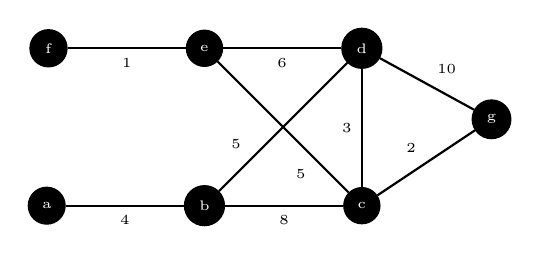
\begin{tikzpicture}[auto, node distance=1.5 cm]
      % Nodes
      \node[terminal] (a) {a};
      \node[terminal] (b) [right=of a] {b};
      \node[terminal] (c) [right=of b] {c};
      \node[terminal] (d) [above =of c] {d};
      \node[terminal] (e) [left=of d] {e};
      \node[terminal] (f) [left=of e] {f};
      \node[terminal] (g) [above right=0.75 and 1.3 of c] {g};
      % Edges
      \begin{scope}[every edge/.style={draw=black, thick}]
        \draw (a) edge node[below]{4} (b);
        \draw (b) edge node[near start]{5} (d);
        \draw (b) edge node[below]{8} (c);
        \draw (c) edge node{3} (d);
        \draw (c) edge node{2} (g);
        \draw (c) edge node[near start]{5} (e);
        \draw (d) edge node{6} (e);
        \draw (d) edge node{10} (g);
        \draw (e) edge node{1} (f);
      \end{scope}
    \end{tikzpicture}
    \caption{The graph $G$ with edge costs.}\label{fig:mtp:01:g}
  \end{subfigure}
  \begin{subfigure}[b]{0.47\linewidth}\centering
    \footnotesize
    \begin{tabular}{r||c|c|c|c|c|c|c}
 $d_{ij}$ & $a$ & $b$ & $c$ & $d$ & $e$ & $f$ & $g$ \\ \hline\hline
      $a$ &  0  &  5  &  8  &     &     &  6  &     \\ \hline
      $b$ &  2  &  0  &  2  &  2  &     &     &     \\ \hline
      $c$ &     &     &  0  & 10  &  4  &     &  1  \\ \hline
      $d$ &     &  3  &     &  0  &  6  &     &  2  \\ \hline
      $e$ &     &     &     &     &  0  &     &     \\ \hline
      $f$ &  2  &  8  &     &     &  5  &  0  &     \\ \hline
      $g$ &     &     &  5  &  5  &     &     &  0
    \end{tabular}
    \caption{The assignment cost function $d$.}\label{fig:mtp:01:d}
    \end{subfigure}
  \caption{Instance of the \gls{mtp} problem.}
  \label{fig:mtp:01}
\end{figure}

Figure~\ref{fig:mtp:01} shows an example of the \gls{mtp} represented as a graph
(Figure~\ref{fig:mtp:01:g}) taken from our recurring example (Figure~\ref{fig:pcstp:01})
and an assignment function (\ref{fig:mtp:01:d}) for which the values have been
chosen arbitrarily.
Figure~\ref{fig:mtp:01:opt}
shows the optimal solution
$$T = ( \{ c, e, f, g \}, \{(c, e), (c, g), (e, f)\})$$
to this problem with total cost
$$c(T) = (1 + 5 + 2) + (6 + 2 + 2) = 18\mathnormal{.}$$
\begin{figure}[h!]
  \centering
      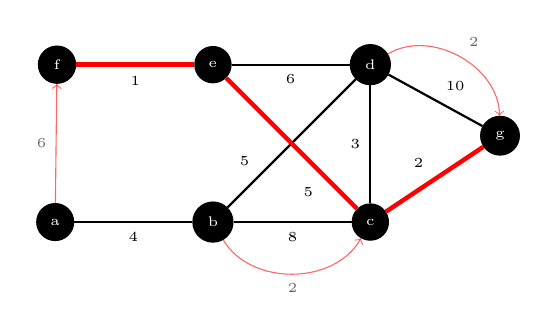
\begin{tikzpicture}[auto, node distance=1.5 cm]
      % Nodes
      \node[terminal] (a) {a};
      \node[terminal] (b) [right=of a] {b};
      \node[terminal] (c) [right=of b] {c};
      \node[terminal] (d) [above =of c] {d};
      \node[terminal] (e) [left=of d] {e};
      \node[terminal] (f) [left=of e] {f};
      \node[terminal] (g) [above right=0.75 and 1.3 of c] {g};
      % Edges
      \begin{scope}[every edge/.style={draw=black, thick}]
        \draw (a) edge node[below]{4} (b);
        \draw (b) edge node[near start]{5} (d);
        \draw (b) edge node[below]{8} (c);
        \draw (c) edge node{3} (d);
        \draw (c) edge[selected] node{2} (g);
        \draw (c) edge[selected] node[near start]{5} (e);
        \draw (d) edge node{6} (e);
        \draw (d) edge node{10} (g);
        \draw (e) edge[selected] node{1} (f);
      \end{scope}
      \begin{scope}[every edge/.style={assignment}]
        \draw[->] (a) edge node{6} (f);
        \draw[->] (b) edge[bend right=60] node[below]{2} (c);
        \draw[->] (d) edge[bend left=60] node{2} (g);
      \end{scope}
    \end{tikzpicture}
    \caption{Optimal solution to the \gls{mtp} problem in Figure~(\ref{fig:mtp:01}).
      The edges of the facility are coloured in red and assignments are denoted with translucent red arrows.}\label{fig:mtp:01:opt}
  \end{figure}

  Since there exists a relative balance between the cost of the edges in the graph and the assignment cost, $T$
  only spans part of the graph. This raises a point. As assignment costs tend to infinity, the \gls{mtp} begins to look
  like the Minimum Spanning Tree problem.
  This is akin to the \gls{stp} with $N = V$ and the \gls{pcstp} with infinite prize
  on all vertices. However, when edge costs tend toward infinity, the facility will naturally become a single vertex
  and the \gls{mtp} will begin to look like the $1$-Median problem (See Section~\ref{sec:related:median}).

\paragraph{Reduction from the Prize-Collecting Steiner Tree Problem}
Instances of the \gls{pcstp} can straightforwardly be reduced to instances of the \gls{mtp}. This is in exact correspondence to how instances
of the \gls{ptp} can be reduced to instances of the Median Tour Problem (Section~\ref{sec:related:median}).
Given an instance of the \gls{pcstp} on graph $G = (V, E, c, p)$, define the assignment cost function

$$d_{ij} =
 \begin{cases}
   0 & i = j \\
   p_i & i \neq j
 \end{cases}\mathnormal{.}
 $$
 then solving the \gls{mtp} on the graph $G' = (V, E, c, d)$ is equivalent to solving the \gls{pcstp} on $G$. Since every vertex assignment not
 to the vertex itself pays the \textit{prize} of that vertex, every vertex not in the facility will pay its prize as penalty. Hence,
 any solution $T = (V, E, c, p)$ to the \gls{pcstp} on $G$ will have the exact same cost as the solution $T' = (V, E, c, d)$ to the \gls{mtp} on $G'$.

\begin{figure}[h]\centering
  \begin{subfigure}[b]{0.47\linewidth}\centering
    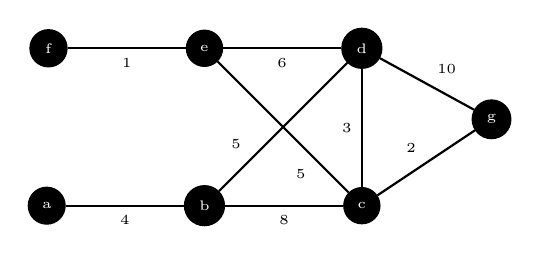
\begin{tikzpicture}[auto, node distance=1.5 cm]
      % Nodes
      \node[terminal] (a) {a};
      \node[terminal] (b) [right=of a] {b};
      \node[terminal] (c) [right=of b] {c};
      \node[terminal] (d) [above =of c] {d};
      \node[terminal] (e) [left=of d] {e};
      \node[terminal] (f) [left=of e] {f};
      \node[terminal] (g) [above right=0.75 and 1.3 of c] {g};
      % Edges
      \begin{scope}[every edge/.style={draw=black, thick}]
        \draw (a) edge node[below]{4} (b);
        \draw (b) edge node[near start]{5} (d);
        \draw (b) edge node[below]{8} (c);
        \draw (c) edge node{3} (d);
        \draw (c) edge node{2} (g);
        \draw (c) edge node[near start]{5} (e);
        \draw (d) edge node{6} (e);
        \draw (d) edge node{10} (g);
        \draw (e) edge node{1} (f);
      \end{scope}
    \end{tikzpicture}
    \caption{The graph $G$ with edge costs.}
    \label{fig:mtp:pcstp:g}
  \end{subfigure}
  \begin{subfigure}[b]{0.47\linewidth}\centering
    \footnotesize
    \begin{tabular}{r||c|c|c|c|c|c|c}
 $d_{ij}$ & $a$ & $b$ & $c$ & $d$ & $e$ & $f$ & $g$ \\ \hline\hline
      $a$ &  0  &  12 &  12 &  12 &  12 &  12 &  12 \\ \hline
      $b$ &  0  &  0  &  0  &  0  &  0  &  0  &  0  \\ \hline
      $c$ &  0  &  0  &  0  & 0  &  0  &  0  &  0  \\ \hline
      $d$ &  10 &  10 &  10 &  0  &  10 &  10 &  10 \\ \hline
      $e$ &  0  &  0  &  0  &  0  &  0  &  0  &  0  \\ \hline
      $f$ &  0  &   0 &  0  &  0  &  0  &  0  &  0  \\ \hline
      $g$ &  3  &   3 &  3  &  3  &  3  &  3  &  0
    \end{tabular}
    \caption{The assignment cost function $d$.}
  \end{subfigure}

  \begin{subfigure}[b]{0.60\linewidth}\centering
    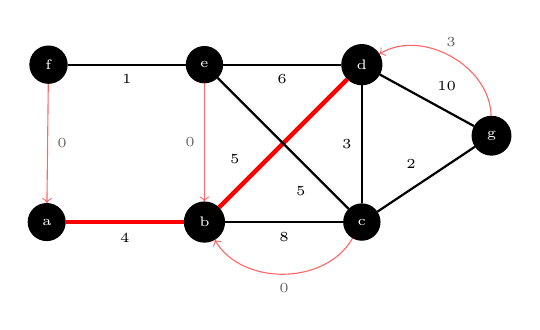
\begin{tikzpicture}[auto, node distance=1.5 cm]
      % Nodes
      \node[terminal] (a) {a};
      \node[terminal] (b) [right=of a] {b};
      \node[terminal] (c) [right=of b] {c};
      \node[terminal] (d) [above =of c] {d};
      \node[terminal] (e) [left=of d] {e};
      \node[terminal] (f) [left=of e] {f};
      \node[terminal] (g) [above right=0.75 and 1.3 of c] {g};
      % Edges
      \begin{scope}[every edge/.style={draw=black, thick}]
        \draw (a) edge[selected] node[below]{4} (b);
        \draw (b) edge[selected] node[near start]{5} (d);
        \draw (b) edge node[below]{8} (c);
        \draw (c) edge node{3} (d);
        \draw (c) edge node{2} (g);
        \draw (c) edge node[near start]{5} (e);
        \draw (d) edge node{6} (e);
        \draw (d) edge node{10} (g);
        \draw (e) edge node{1} (f);
      \end{scope}
      \begin{scope}[every edge/.style={assignment}]
        \draw[->] (c) edge[bend left=60] node{0} (b);
        \draw[->] (e) edge node[left]{0} (b);
        \draw[->] (f) edge node{0} (a);
        \draw[->] (g) edge[bend right=60] node[above]{3} (d);
      \end{scope}
    \end{tikzpicture}
    \caption{Optimal Solution to (\ref{fig:mtp:pcstp:g}).}
  \end{subfigure}

  \caption{Instance of the \gls{pcstp} (Figure~\ref{fig:pcstp:01}) with optimal solution.}
  \label{fig:mtp:pcstp}
\end{figure}

Figure~\ref{fig:mtp:pcstp} shows how this reduction works on the \gls{pcstp} instance in Figure~\ref{fig:pcstp:01}
as well as the optimal solution
$$T = (\{a,b,d\}, \{(a,b), (b,d)\})$$
with cost
$$c(T) = (4 + 5) + (3) = 12$$
which is the same cost as the optimal solution to the original \gls{pcstp} problem (Figure~\ref{fig:pcstp:01:opt}).

While it is obvious that the \gls{mtp} problem is NP-hard -- something which has already been established in previous literature
 (See Section~\ref{sec:related:median}) -- this reduction again implies the NP-hardness of the problem.
 \section{Applications}
 We expect the \acrlong{mtp} to have similar applications to the \gls{pcstp} as they are fairly similar problems.

 Foremost, any kind of problem which involves a two tiered supply system could possibly be modelled as an instance of the
 \gls{mtp}. Take, for example, the placement of postal warehouses --- building and staffing a new warehouse comes at
 a cost but makes easier the delivery of packages to the surrounding area. The cost of warehouses (and the cost of maintaining
 a transport networks between them) could be modelled as edge costs, while the cost of delivering post from a warehouse to an area
 could be modelled as assignment costs.  Similar scenarios could exist in water supply, military supply lines, aid distribution etc.

 Another area of interest may be within computation biology, which as seen applications for the \gls{pcstp} and similar
 \citep{sun2018classical, akhmedov2016divide}.
\section{Integer Programming Formulation}

Given an instance of the \gls{mtp} as defined above,
Formulation~(\ref{form:mtp:cut}) is an \gls{ilp} formulation of the \gls{mtp}.
It is loosely inspired by the one defined by \citet{lucena2004strong}
(Formulation~\ref{form:lower:gsec}, Section~\ref{sec:lower:gsec}) for the Prize-Collecting
Steiner Tree Problem.

The variables $\bd x$ and $\bd y$ are boolean
decision vectors which are interpreted as follows.
As with the \gls{pcstp} formulation, when $x_{ij} = 1$,
the edge between vertices $v_i$ and $v_j$ is part of the solution -- note that only
one of $x_{ij}$ and $x_{ji}$ are variables in model and we will use both indices interchangably
to refer to the same variable for the sake of readability.

Similarly, $\bd y$ describes the assignment relation of a solution. When
$y_{ij} = 1$, vertex $v_i$ is \textit{assigned} to vertex $v_j$ and the corresponding
assignment cost must be paid.
These relations are reflected in the objective function.
When $y_{kk} = 1$, we consider that vertex assigned to
itself, which implies that vertex $v_k$ is part of the facility.

 \begin{formulation}[h!]
   \begin{subequations}
     \begin{alignat}{3}
       &\underset{\bd x, \bd y}{\text{minimize}}
       & & \sum_{ij \in E} c_{ij} x_{ij} +  \sum_{i, j \in V} d_{ij}y_{ij}  & \\
       & \text{subject to}\quad
       & & \sum_{ij \in E} x_{ij} = \sum_{i \in V} y_{ii} - 1 &&  \label{form:mtp:tree}\\
       &&& x(E(S)) \leq \sum_{i \in S \setminus \{s\}} y_{ii}
       && \forall S \subseteq V, s \in S \label{form:mtp:gsec} \\
       &&& \sum_{j \in V} y_{kj} = 1 && \forall k \in V \label{form:mtp:assignment}\\
       &&& y_{ik} \leq  y_{kk}
       && \forall i, k \in V \label{form:mtp:facility}\\
       &&& y_{kk} \leq \sum_{i \in \gls{delta}(k)} x_{ik}
       && \forall k \in V \label{form:mtp:legal} \\
       &&& \bd x \in \BB^{|E|} && \\
       &&& \bd y \in \BB^{|V \times V|}
     \end{alignat}\label{form:mtp:cut}
   \end{subequations}
   \caption{\gls{ilp} formulation of the \gls{mtp}.}
 \end{formulation}

 Since edges have nonnegative weights, we know that the shape of the facility must be a tree.
 Constraint (\ref{form:mtp:tree}) ensures that any facility has exactly one less edge than
 vertices, and constraints (\ref{form:mtp:gsec}) ---commonly known as \glspl{gsec}
 ---ensures that no subset of vertices in the facility can form
 a cycle. Together, these ensure that any feasible
 solution must be a single, connected subgraph of $G$
 which is shaped as a tree.

 The rest of the constraints are concerned with making sure that every vertex in $G$ is
 assigned to a vertex in the facility in any feasible solution. Constraint
 (\ref{form:mtp:assignment}) ensures that every vertex in $G$ is assigned to exactly one
 vertex, and constraint (\ref{form:mtp:facility}) ensures that a vertex can only be assigned
 to if it is part of the facility. This could alternatively be modelled as
 $$\sum_{i \in V} y_{ik} \leq  M y_{kk}  \qquad \forall i \in V$$
 for some $M \gg |V|$.

 Finally, the constraints (\ref{form:mtp:legal}) ensure that no vertex can feasibly be part
 of the facility unless an edge in its adjacency is selected -- that is, unless it is spanned
 by the solution tree.

 \paragraph{Valid Inequalities}
 Whenever a vertex is connected to the facility, it trivially must be assigned to itself. This
 follows directly from the fact that $d_{ii} = 0$ for all $i \in V$ and thus have $d_{ij} \geq d_{ii}$
 for all $j \in V$. The fact that this is implied by the probe (i.e. it is always correct to assign a
 vertex in the facility to itself) allows us to not formalise it in the problem. However, we can
 still add the constraints
 \begin{equation}\label{form:mtp:str}
 y_{ii} \geq x_{ji} \qquad \forall i \in V,  \forall j \in \delta(i)
\end{equation}
 to as valid constraints to formalise this relation.

 Similar to how \citeauthor{ljubic2005solving} constrain the degree of Nonterminals in Constraint
 (\ref{form:exact:strength}), the same idea holds for the \gls{mtp} but in a slightly different manner.
 Consider the set of vertices which cost nothing to assign and cannot be assigned to as \textit{Nonterminals},
 $$N = \left\{ i \in V \middle\vert \sum_{j \in v} d_{ij} = 0 \wedge  \forall j. d_{ji} = \infty\right\}\mathnormal{.}$$
 As nonterminals play no part in the assignment question, they cannot be a leaf node in an optimal solution as they could trivially
 be removed from the facility to produce a solution with no greater cost. Thus they
 must have degree of at least
 two should they be part of an optimal facility, and it is valid to add the constraint
 \begin{equation}\label{mtp:valid:deg}
   \sum_{j \in \delta(i)}x_{ij} \geq 2 x_{ik} \qquad \forall i \in N, \: \forall k \in \delta(i)
 \end{equation}
 to the model. The intuitive interpretation of (\ref{mtp:valid:deg}) is that if any edge adjacent to
 a nonterminal is selected, \textit{at least} two edges adjacent to the nonterminal must be selected.
\section{Solver}\label{sec:mtp:solver}
As mentioned previously, to test out the applicability of some of the methods introduced in
the Chapter~\ref{chap:solving}, we have implemented a solver for the \gls{mtp}.
This section both goes over algorithmic and technical implemention details of the solver

The solver makes use of the general purpose \gls{mip} solver
Gurobi \citep{gurobi} (version 8.0.1)
and its Python 3 interface. While this means that the callbacks written for the solver
will naturally have much slower performance than if, for example, we had chosen to make
use of the C or C++ interface, the Python interface was chosen for its higher level interface
and better ease-of-use -- giving better iteration times. Having no other computational results
to compare against, this trade-off was easy to make.

The Python library,
NetworkX\footnote{\url{https://networkx.github.io/}} \citep{hagberg2008exploring}
was used for the internal graph representation of the
problem instances in the solver as well as for implementation of common
graph algorithms. It is worth noting that NetworkX features algorithm implementations
in native Python instead of the more efficient Python C modules. This, again, has some
performance implications especially with regards to user callbacks (which we will
 touch on below).

The source code of the solver as well as the benchmark suite
can be found on GitHub\footnote{\url{https://github.com/wsprent/thesis-code}}.

\paragraph{Preprocessing}

While we have seen that preprocessing for the \gls{pcstp} is a \textit{very} important
tool in solving hard instances, our solver does not include any preprocessing routines.

This is not a design choice but rather a limitation. The \gls{mtp} is
more combinatorially
complex than the \gls{pcstp} which makes it impossible to directly translate those particular
methods. Where removing an edge or a vertex in the \gls{pcstp}
has very straightfoward consequences in
some cases, it may have cascading effects in the \gls{mtp}.

We have simply yet to uncover which preprocessing routines can be applied to instances of
the \gls{mtp}.

\paragraph{Branch and Cut}
The choice of applying a branch and cut method in the solver, is fairly straight
forward to make as it is infeasible to load all of the exponential number of
\glspl{gsec} into the model initially. Thus, the solver
\textit{must} make use of
Gurobi's \textit{Lazy Constraints} to avoid producing infeasible solutions
and \textit{may} additionally make use of \textit{User Cuts} to potentially
give faster runtimes by producing tighter lower bounds.

Both of these are included in the solver through Gurobi's callback system.
\subparagraph{Lazy Constraints}
The job of the lazy constraint callback involves separating integer solutions
which violate any \glspl{gsec}. This boils down to finding cycles in the solution
graph.

Given an integer solution $(\bd{\hat{x}}, \bd{\hat{y}})$ produced by Gurobi, we
identify any violated \glspl{gsec} by first generating a NetworkX graph,
$$S = (\{i \in V \mid \hat y_{ii} = 1 \}, \{ (i, j) \in E \mid \hat x_{ij} = 1\})\mathnormal{.}$$
Then we again use NetworkX to find all simple cycles in $S$. Then for each vertex
subsets $C \subseteq V$ induced by a cycle
in $S$, we add all of the violated constraints
$$x(E(C)) \leq y_{ii} \setminus \{c\} \qquad \forall c \in C$$
to the model.
\subparagraph{User Cuts}
The callback responsible for
Separating infeasible LP solutions with regards to \glspl{gsec}
have been adapted for the solver from the max-flow/min-cut  method used by \citet{lucena2004strong}
 (see Section~\ref{sec:solving:lower})
-- and later \citet{ljubic2005solving} and \citet{gamrath2017scip} -- for the \gls{pcstp}.

Adapting this separation procedure can be done directly. Having the decision variable
$\hat y_{ii} = b$ for some $b \in [0,1]$ in the LP relaxation of
the \gls{mtp} corresponds directly to $\hat y_i = b$ with respect to the \glspl{gsec}.
Once again, we use NetworkX to both represent the support graph and solve max flow problem(s).

As with the DHEA solver by \citet{ljubic2005solving}, we allow for controlling the maximum amount
of cuts performed at each node in the b\&b tree
with a \texttt{-{}-max-cuts} option. Additionally, this can be set
to \texttt{0} to disable the user cut routine altogether.

\paragraph{Primal Heuristics}
The solver an optional custom primal heuristic adapted from the primal hueristics detailed
for the \gls{pcstp} by \citet{ljubic2005solving}
(see Sections \ref{sec:solving:exact} and , \ref{sec:heuristics:lp}).

As with the cuts above, we exploit the fact that $y_i$ in the \gls{pcstp}
corresponds directly to $y_{ii}$ in the \gls{mtp}.

One thing we have not adapted, however, is the last step of solving the \gls{mtp}
on the final tree. This is left for further research.

The primal heuristic can be disabled in favour of Gurobi's inbuilt heuristic with
the switch $$\texttt{-{}-no-heuristics}\mathnormal{.}$$
\section{Computational Experience}
With having no prior attempts to solve the \gls{mtp} in the general case to draw from,
we have no interesting timings to test our model against nor any previously constructed
datasets to perform benchmarks on. Thus, we present in this section two things,
\begin{enumerate}
\item The specifics of how we have generated a new dataset for the \gls{mtp} out of previously released,
  as well as the details of the dataset, and
\item The result of performing benchmarks testing the effectiveness of
  \begin{enumerate*}[label={\alph*)}, font=\bfseries]
  \item our primal heuristic,
  \item the user cut routine, and
  \item the extra constraint (\ref{form:mtp:str}).
  \end{enumerate*}
\end{enumerate}
In short, we are looking to test out our additions to a what could be called a ``default'' Gurobi
implementation of the \gls{mtp}.

First we will give an overview of the dataset followed by an inspection of the three experiments we have
 performed.
 \subsection{Datasets}
 To perform realistic and relevant benchmarks of the settings in our solver, we need to run the solver
 against instances of the \gls{mtp} which are large enough to not be presolved and preferably small
 enough to solve to optimality within a reasonable timeframe. At the same time, as this is an introduction
 to the problem, we want the instances to be generic, opposed to modelling some specfic application or
 flavour of the \gls{mtp}.

 In getting to this point, our starting point is the \texttt{JMP} dataset presented by 
 \citet{Johnson:2000:PCS:338219.338637}. This was picked mainly for featuring the smallest
 and easiest to solve instances of the \gls{pcstp} instances available
 (and yet -- as shown below -- we have had to truncate the instances).
 The input instances are distributed in the \texttt{STP} format used by the \textit{SteinLib}
 library \citep{koch2001steinlib}.

 The \gls{mtp} instances we output are described in \texttt{STP} format with a small extension.
 This involves the addition of a new \texttt{Section} named \texttt{AssignmentCosts} each line
 in this section describes the cost of assigning a single vertex to another.

 Formally, each line has the format,
 \begin{grammar}
   <assignment> := `D' `\ ' <vertex-id> `\ ' <vertex-id> `\ ' <cost>
 \end{grammar}
 where \textit{<vertex-id>} is an integer id which corresponds to a vertex declared in the \texttt{Graph}
 section of the same file, and \textit{<cost>} is a non-negative real number.

 For example, the following example reads as \textit{the cost of assigning vertex ``1'' to vertex ``2'' is $4.5$.}
\begin{verbatim}
D 1 2 4.5
\end{verbatim}
Appendix \ref{app:report:stp} shows Figure~\ref{fig:mtp:01} represented in the extended STP format.
 \paragraph{Translation}
 In translating the \gls{pcstp} instances into \gls{mtp} instances, we keep all the of the graph
 structure including the edge costs. Hence we only need to generate a set of assignment costs which
  \textit{balanced} with respect to edge costs.

 To generate assignment costs, we first assign any nonterminal with no prize a prize
 equal to the average prize across all vertices. For each vertex, $i$, the cost to assign
 it to some vertex, $j$, is then,
 $$d_{ij} =
 \begin{cases}
   p_i \cdot \frac{sp(i, j)}{\sum_{l \in V}sp(i,l) / |V|} & p_i > 0 \\
      \frac{\sum_{l \in V} p_l}{|V|} \cdot \frac{sp(i, j)}{\sum_{l \in V}sp(i,l) / |V|} & p_i = 0
 \end{cases}\mathnormal{.}
$$
 In other words, vertex $i$'s prize is factored by ratio between length of the shortest path
 between $i$ and $j$ relative to the average distance between vertex $i$ and all vertices.
 This keeps the prizes in the original dataset relevant, and makes ``closeness'' between
 verties with respect to assignment costs somewhat transitive.

 A facet --- perhaps a weakness --- of this method is that it produces somewhat uniform
 assignment costs, and that it requires a connected graph to produce an \gls{mtp} instance
 with a lower-than-infinity optimal value. Furthermore, on connected graphs, all vertices
 are assignable to all vertices, and no vertex is assignable to another vertex at no cost.

 Some of the instances in the \texttt{JMP} dataset are disconnected. For these instances,
 before performing the above, we connect the graph by selecting a random pair of vertices,
 $i,j$, from disjoint components. The edge $(i,j)$ is then added to the edge set with cost
 $$c_{ij} = \sum_{k \in \delta(i)} c_{ik} / |\delta(i)|\mathnormal{.}$$

 The summarise, the output dataset features instances which have connected graphs with
 \textit{smooth} -- as opposed to erratic -- assignment cost functions. All vertices
 can be assigned to all other vertices without incurring infinite cost, and no vertex
 can be assigned to another vertex at zero cost. 

 \paragraph{Truncation} However, even though we chose the ``easiest'' of the available datasets,
 our solver still struggle with our translated instances, and would require a timeout
 value too large time constraint wise.

 Thus we have chosen to create smaller instances by truncating the translated \texttt{JMP}
 instances. The translated dataset mainly contains instances with either $100$ or $400$ vertices,
 and we truncate these into instances containing $60$ and $80$ vertices respectively.

 We accomplish this by iteratively contracting randomly selected edges. To avoid generating a
 vastly more connected graph, we then remove adjacent edges from the resulting vertex until
 we have $|\delta(i)| \frac{n_{target}}{|V|}$ edges in its adjacency (where $i$ is the vertex
 and $n_{target}$ is the number of vertices in the truncated instance) or until we randomly select
 an edge which would disconnect the graph.

 This method is admittedly rather arbitrary, but it aims to accomplish a graph containing similar
 connectivity as well as introducing a level of randomness to ---hopefully--- avoid a too uniform graph.

 The end result from the above is two sets of instances, \texttt{JMP-60} and \texttt{JMP-80}, named
 after the original dataset and the amount of vertices they contain.
 
 \subsection{Experiments}

 To perform our three experiments, we have developed a small rudimentary benchmarking suite. The solver
 itself is equipped with the ability to time itself and perform repeated solving of the same problem.
 For each problem instance, the solver is run with a \texttt{-{}-timeout} of five minutes. This timeout
 is passed directly to Gurobi, so the actual timeout is five minutes plus the time it takes to load the
 graph etc. Each instance is solved five times (the problem is loaded from file each of the five times)
 and the all times reported below is the mean these five timings.

 Executions are grouped by instance, that is for each instance, the solver is run with the following
 settings in order:
 \begin{enumerate}
 \item No user cuts (\texttt{-{}-max-cuts 0 -{}-no-heuristics}).
 \item Maximum of one cut per node (\texttt{-{}-max-cuts 1 -{}-no-heuristics}).
 \item Maximum of 25 cuts per node (\texttt{-{}-max-cuts 25 -{}-no-heuristics}).
 \item Default settings.
 \item With constraint~(\ref{mtp:valid:deg}) (\texttt{-{}-strengthen -{}-no-heuristics}).
 \end{enumerate}
 Grouping benchmarks by instances was done to hopefully improve the chances of each run happening
 under the same circumstances while the precise ordering of the settings is arbitrary.
 
 Default settings solves the input problem on the basic model (Formulation~\ref{form:mtp:cut})
 with a maximum of 25 user cuts, and performs the primal heuristics defined above at every
 25th node.

\textit{System info}

\paragraph{Heuristics}
In this experiment, we look at the performance of our primal heuristic, defined above, versus
the inbuilt heuristic from Gurobi. While the Gurobi heuristic, which is based on rounding
of the the LP solution, has the advantages of being written in a systems programming language
with less overhead and ---probably--- has hooks directly into the core optimiser,
implementing a strong heuristic for the \gls{mtp} should be able to out perform it.

In the case of this particular formulation of the \gls{mtp},
for example, the Gurobi optimiser does not have access to the
many \glspl{gsec}, making it prone to produce infeasible solutions which waste time.

However, our heuristic is rudimentary, adapted directly from a neighbouring problem,
and implemented in an interpreted language. It may struggle to keep up.

For our benchmarks, we have kept the default Gurobi setting of approximately running
the default heuristic $5\%$ of the time when enabled. Our heuristic instead runs on
every 25th node.

\begin{table}[h!]
  \centering
  \begin{tabular}[h!]{|c|c|c|c|c|}\hline
    \multirow{2}{*}{Instance} & \multicolumn{2}{|c|}{$t(s)$} & \multirow{2}{*}{$GAP$} & \multirow{2}{*}{$OPT$} \\
 & Gurobi & Custom &  &  \\\hline
 \hline
 & \multicolumn{2}{|c|}{JMP-60} &  \\\hline
K100 & $\mathbf{134.71}$ & $211.89$ & $\mathbf{0.00\%}$ & $92817.00$ \\
K100.1 & $\mathbf{74.202}$ & $135.37$ & $\mathbf{0.00\%}$ & $95464.00$ \\
K100.10 & $\mathbf{27.155}$ & $41.159$ & $\mathbf{0.00\%}$ & $87948.00$ \\
K100.2 & $251.31$ & $\mathbf{230.57}$ & $\mathbf{0.00\%}$ & $143559.00$ \\
K100.3 & $\mathbf{28.241}$ & $36.64$ & $\mathbf{0.00\%}$ & $72582.00$ \\
K100.4 & $\mathbf{6.4068}$ & $8.0836$ & $\mathbf{0.00\%}$ & $60398.00$ \\
K100.5 & $\mathbf{17.3}$ & $22.141$ & $\mathbf{0.00\%}$ & $77180.00$ \\
K100.6 & $\mathbf{75.976}$ & $84.69$ & $\mathbf{0.00\%}$ & $91351.00$ \\
K100.7 & $253.38$ & $\mathbf{204.83}$ & $\mathbf{0.00\%}$ & $142316.00$ \\
K100.8 & $\mathbf{223.06}$ & $246.2$ & $\mathbf{0.00\%}$ & $125996.00$ \\
K100.9 & $\mathbf{9.6662}$ & $11.188$ & $\mathbf{0.00\%}$ & $59640.00$ \\
 \hline
 \hline
 & \multicolumn{2}{|c|}{JMP-80} &  \\\hline
K400 & $\mathbf{28.829}$ & $46.232$ & $\mathbf{0.00\%}$ & $71261.00$ \\
K400.1 & $\mathbf{49.622}$ & $105.36$ & $\mathbf{0.00\%}$ & $75102.00$ \\
K400.10 & $\mathbf{33.672}$ & $48.309$ & $\mathbf{0.00\%}$ & $68481.00$ \\
K400.2 & $72.454$ & $\mathbf{70.31}$ & $\mathbf{0.00\%}$ & $71194.00$ \\
K400.3 & $\mathbf{28.254}$ & $50.354$ & $\mathbf{0.00\%}$ & $62110.00$ \\
K400.4 & $23.342$ & $\mathbf{20.953}$ & $\mathbf{0.00\%}$ & $68898.00$ \\
K400.5 & $\mathbf{87.756}$ & $166.34$ & $\mathbf{0.00\%}$ & $84188.00$ \\
K400.6 & $35.959$ & $\mathbf{30.579}$ & $\mathbf{0.00\%}$ & $52623.00$ \\
K400.7 & $104.45$ & $\mathbf{100.75}$ & $\mathbf{0.00\%}$ & $84901.00$ \\
K400.8 & $\mathbf{20.78}$ & $30.11$ & $\mathbf{0.00\%}$ & $61355.00$ \\
K400.9 & $\mathbf{13.676}$ & $13.799$ & $\mathbf{0.00\%}$ & $57636.00$ \\
 \hline

%%%
%%% Local Variables:
%%% TeX-master: "report"
%%% reftex-default-bibliography: ("lit.bib")
%%% End:
    

  \end{tabular}
  \caption{Timing results for the primal heuristic benchmark. The
    \textbf{bolded} times are the fastest.}
  \label{tab:jmp:heuristics}
\end{table}

In Table~\ref{tab:jmp:heuristics} we show the timings of running the heuristics experiment.
In both cases, all instances were solved to optimality within the five minute time limit, which
is shown by the $\mathbf{0\%}$ $GAP$ between the highest lower bound and best incumbent.
The results are somewhat mixed, with the Gurobi heuristic proving to be faster in the majority
of cases. In a couple of cases, particularly instances \texttt{K400.1} and \texttt{K400.5},
our primal heuristic is twice as slow as the Gurobi heuristic. The picture of having the
custom primial heuristic only sometimes being worthwhile mirrors results from
\citet{ljubic2005solving}, who experienced the same ambivalent results for their solver.

While these results suggest that turning off the Python-based heuristic is the way to go
in most cases,
they also suggest that perhaps by improving the heuristic we can achieve performance
which eclipses the default performance.

How we should achieve this, depends heavily on which way the heuristic is ``underperforming''.
 Is it producing solutions of too high value? Is it running too slowly?

 If speed is a problem, a good first option to improve performance,
 would be to rewrite the heuristic procedure
in a systems programming language (e.g. C, C++, Rust).
This should by default give a multi-factor speedup, and gives better options for
later performance optimisation.

If the heuristic isn't producing good enough solutions, then we could look at the final step
of the algorithm. In our implementation we do not solve the \gls{mtp} on the final tree contrary
to the original algorithm defined by \citet{ljubic2005solving}. It may be that by skipping
this step, we are missing out on a lot.

In both cases, simply running the heuristic on every 25th node is not a very cunning
way of using our resources, and there is no reason to believe that this achieves optimal
performance. If the heuristic was reimplemented to be blazingly fast, it may be advisable to
simply run the full heuristic at every node of the branch and bound tree
(which mirrors what we have seen in Section~\ref{sec:solving:exact}). However, it may also
be a good idea to change behaviour based on the nature of the LP solution, either by
running a different heuristic when the LP solution far from integral or \textit{only}
running the heuristic when the solution is close to integral. 

Either way, our results seem to confirm that reusing the heuristic from
\citeauthor{ljubic2005solving} is not a faulty strategy, and that the \gls{pcstp}
and \gls{mtp} similar enough for knowledge sharing.

\paragraph{User Cuts}
A very different story is told by our user cuts experiment. Table~\ref{tab:jmp:maxcut}
displays the results of our user cut experiment. The results are very clear, the performance
of our user cut routine is atrocious compared to disabling it altogether. In most instances
we see more than a $10 \times$ slowdown for the MC-25 configuration compared to the MC-0
configuration, with the differential peaking for instance \texttt{K100.2} at around $30 \times$.

These results also shown the only example of our solver not being able to solve an instance
within the given time limit. Instance \texttt{K100.8} proves too difficult for the solver
given the default \texttt{-{}-max-cuts 25} setting, causing it to terminate on average with
a LP/incumbent gap of $6.52\%$.

Such stark differences between configurations
raise the question of whether or not we are talking about a performance
related bug in the implementation of the user cut routine.
While this may be the case, we will proceed as if it is not.

\begin{table}[h!]
  \centering
  \begin{tabular}[h!]{|c|c|c|c|c|c|}\hline
    \multirow{2}{*}{Instance} & \multicolumn{3}{|c|}{$t(s)$} & \multirow{2}{*}{$OPT$} \\
 & MC-0 & MC-1 & MC-25 &  \\\hline
 \hline
 & \multicolumn{3}{|c|}{JMP-60} &  \\\hline
K100 & $\mathbf{12.607}$ & $68.296$ & $\mathit{(5.06\%)^*}$ & $96746.00$ \\
K100.1 & $\mathbf{2.7232}$ & $5.3032$ & $34.663$ & $78044.00$ \\
K100.10 & $\mathbf{48.276}$ & $106.4$ & $\mathit{(19.07\%)^*}$ & $106766.00$ \\
K100.2 & $\mathbf{2.1829}$ & $6.7152$ & $19.502$ & $90898.00$ \\
K100.3 & $\mathbf{42.662}$ & $124.82$ & $\mathit{(20.21\%)^*}$ & $69654.00$ \\
K100.4 & $\mathbf{2.4715}$ & $2.7063$ & $20.619$ & $60837.00$ \\
K100.5 & $\mathbf{30.486}$ & $60.194$ & $\mathit{(11.17\%)^*}$ & $98802.00$ \\
K100.6 & $\mathbf{58.847}$ & $132.78$ & $\mathit{(16.46\%)^*}$ & $124135.00$ \\
K100.7 & $\mathbf{6.8507}$ & $19.073$ & $90.602$ & $78161.00$ \\
K100.8 & $\mathbf{29.964}$ & $86.204$ & $\mathit{(5.01\%)^*}$ & $140414.00$ \\
K100.9 & $\mathbf{1.5633}$ & $3.6496$ & $14.176$ & $67353.00$ \\
 \hline
 \hline
 & \multicolumn{3}{|c|}{JMP-80} &  \\\hline
K400 & $\mathbf{34.112}$ & $54.474$ & $261.57$ & $55277.00$ \\
K400.1 & $\mathbf{135.89}$ & $\mathit{(8.52\%)^*}$ & $\mathit{(28.80\%)^*}$ & $67856.00$ \\
K400.10 & $\mathbf{12.101}$ & $17.978$ & $172.47$ & $53130.00$ \\
K400.2 & $\mathbf{38.536}$ & $131.12$ & $\mathit{(22.85\%)^*}$ & $64848.00$ \\
K400.3 & $\mathbf{15.414}$ & $41.03$ & $\mathit{(6.88\%)^*}$ & $57156.00$ \\
K400.4 & $\mathbf{4.0871}$ & $9.511$ & $22.29$ & $55372.00$ \\
K400.5 & $\mathbf{69.794}$ & $175.37$ & $\mathit{(20.04\%)^*}$ & $91691.00$ \\
K400.6 & $\mathbf{80.716}$ & $\mathit{(6.41\%)^*}$ & $\mathit{(26.01\%)^*}$ & $60830.00$ \\
K400.7 & $\mathbf{21.066}$ & $46.377$ & $\mathit{(3.81\%)^*}$ & $63192.00$ \\
K400.8 & $2.2992$ & $\mathbf{1.8638}$ & $7.8588$ & $46976.00$ \\
K400.9 & $\mathbf{6.9499}$ & $16.587$ & $131.37$ & $55029.00$ \\
 \hline

%%%
%%% Local Variables:
%%% TeX-master: "report"
%%% reftex-default-bibliography: ("lit.bib")
%%% End:
    

  \end{tabular}
  \caption{Timing results for running the user cut experiments. The columns MC-0,
    MC-1, and MC-25 shown the timings for running the solver with no user cuts, max
    one user cut per node, and max 25 user cuts per node respectively.
    \textbf{Bold} font indicates fastest time; \textit{Italic} font indicates
    timeout; the percentage GAP is shown is the highest across the three configurations.}\label{tab:jmp:maxcut}
\end{table}

Having to potentially solve a max-flow problem for each vertex in the input graph incurs a runtime
of $O(n^2 \log n)$. This makes the separation procedure quite costly compared
to our primal heuristic.
Spending this much time in the Python interpreter may actually be enough to explain the performance
disrepancy.

Furthermore, enabling user cuts in Gurobi requires the disabling of the \texttt{PreCrush} setting
which disallows Gurobi from reformulating constraints when presolving the model. This means
that a user cut routine must not just justify itself in terms of time spent versus tigher bounds,
but also with respect to a weakening of the presolving routine.

In the end, these results show that disabling user cuts altogether in our model is definitely
the optimal option.

\paragraph{Strengthening the Model}
Our final experiment involves modifying the model itself instead of behaviour of the Gurobi solver.
This obviously involves a trade off between increasing the size of the model and reducing the size
of the feasible region.

\begin{table}[h!]
  \centering
  \begin{tabular}[h!]{|c|c|c|c|c|}\hline
    \multirow{2}{*}{Instance} & \multicolumn{2}{|c|}{$t(s)$} & \multirow{2}{*}{$GAP$} & \multirow{2}{*}{$OPT$} \\
 & Without (\ref{form:mtp:str}) & With (\ref{form:mtp:str}) &  &  \\\hline
 \hline
 & \multicolumn{2}{|c|}{JMP-60} &  \\\hline
K100 & $\mathbf{124.69}$ & $134.71$ & $\mathbf{0.00\%}$ & $92817.00$ \\
K100.1 & $88.789$ & $\mathbf{74.202}$ & $\mathbf{0.00\%}$ & $95464.00$ \\
K100.10 & $27.249$ & $\mathbf{27.155}$ & $\mathbf{0.00\%}$ & $87948.00$ \\
K100.2 & $\mathbf{244.33}$ & $251.31$ & $\mathbf{0.00\%}$ & $143559.00$ \\
K100.3 & $\mathbf{26.562}$ & $28.241$ & $\mathbf{0.00\%}$ & $72582.00$ \\
K100.4 & $\mathbf{4.0936}$ & $6.4068$ & $\mathbf{0.00\%}$ & $60398.00$ \\
K100.5 & $\mathbf{16.592}$ & $17.3$ & $\mathbf{0.00\%}$ & $77180.00$ \\
K100.6 & $\mathbf{51.721}$ & $75.976$ & $\mathbf{0.00\%}$ & $91351.00$ \\
K100.7 & $\mathbf{222.64}$ & $253.38$ & $\mathbf{0.00\%}$ & $142316.00$ \\
K100.8 & $\mathit{310.65}^*$ & $\mathbf{223.06}$ & $6.52\%$ & $125996.00$ \\
K100.9 & $\mathbf{6.7659}$ & $9.6662$ & $\mathbf{0.00\%}$ & $59640.00$ \\
 \hline
 \hline
 & \multicolumn{2}{|c|}{JMP-80} &  \\\hline
K400 & $\mathbf{28.829}$ & $30.159$ & $\mathbf{0.00\%}$ & $71261.00$ \\
K400.1 & $\mathbf{49.622}$ & $57.839$ & $\mathbf{0.00\%}$ & $75102.00$ \\
K400.10 & $33.672$ & $\mathbf{24.728}$ & $\mathbf{0.00\%}$ & $68481.00$ \\
K400.2 & $72.454$ & $\mathbf{61.184}$ & $\mathbf{0.00\%}$ & $71194.00$ \\
K400.3 & $\mathbf{28.254}$ & $38.885$ & $\mathbf{0.00\%}$ & $62110.00$ \\
K400.4 & $23.342$ & $\mathbf{13.599}$ & $\mathbf{0.00\%}$ & $68898.00$ \\
K400.5 & $87.756$ & $\mathbf{80.723}$ & $\mathbf{0.00\%}$ & $84188.00$ \\
K400.6 & $35.959$ & $\mathbf{27.161}$ & $\mathbf{0.00\%}$ & $52623.00$ \\
K400.7 & $104.45$ & $\mathbf{94.067}$ & $\mathbf{0.00\%}$ & $84901.00$ \\
K400.8 & $\mathbf{20.78}$ & $20.952$ & $\mathbf{0.00\%}$ & $61355.00$ \\
K400.9 & $\mathbf{13.676}$ & $18.678$ & $\mathbf{0.00\%}$ & $57636.00$ \\
 \hline

%%%
%%% Local Variables:
%%% TeX-master: "report"
%%% reftex-default-bibliography: ("lit.bib")
%%% End:
    

  \end{tabular}
  \caption{Timing results with and without constraint constraints~(\ref{form:mtp:str}).
    \textbf{Bold} font indicates fastest time;
    \textit{Italic} font indicates
    timeout; the percentage GAP is shown is the highest across the two configurations.} 
  \label{tab:jmp:strengthen}
\end{table}

Table~\ref{tab:jmp:strengthen} shows the effects of adding constraints~(\ref{form:mtp:str}) to
the model. For most of the instances there is very little difference between the two models
of the problem in how long it takes to reach an optimal solution. Notably, \texttt{K100.8} is
solved in $223$ seconds with the strengthened model yet times out on the basic model at $310$
seconds. The only other stark runtime difference of this caliber is on instance \texttt{K400.4}
which took on average $13.6$ and $23.3$ seconds to solve with and without the extra constraints
respectively.

Either way, we see no clear tendencies in these results. Sometimes adding the extra constraints
pay off in faster runtimes and sometimes it may cause slowdown. Maybe, with extra research, it
would be possible to determine whether certain characteristics in an instance make either option
more desirable.

It would also be interesting to see if disabling user cuts would make a difference with regards
to strengthening the model. As mentioned above, adding user cuts requires disabling part of
Gurobi's presolve. It is not unrealistic that the extra constraints could add something there.
\section{Conclusion}
In this chapter we have taken a look at the \acrlong{mtp}. We have defined the problem as
a graph optimisation problem on an undirected graph and then reformulated it as an \gls{ilp}
problem. As our main contribution, however, we have detailed and implemented a solver for the
problem based on the Gurobi optimisation suite on which we have performed a set of experiments
against a newly generated dataset.

Our new dataset, generated from a dataset for the \gls{pcstp}, comprises 22 instances both in
full and truncated forms (with 100 to 400 and 60 to 80 vertices respectively). This dataset
has been made available on ??? for further use. We have solved all truncated instances to
optimality, but leave the full instances to the reader.

For our solver, we have attempted to translate proven succesful methods for the \gls{pcstp}
into methods for
the \gls{mtp}.
In our experiments, we validated the usefulness of our primal heuristic callback and
a strengthened model to the point where they did not notably decrease performance.
We failed to show the same for our user cut callback, which significantly slowed down the
optimiser.

Based on these results, we are confident that it is possible to directly apply research on
the \gls{pcstp} to the \gls{mtp}. While there are some cases where additonal work must be
done to translate an algorithm ---e.g. the primal heuristic for which we skipped a step---
it seems that the problems are either generic enough or similar enough for information share.

For further work, it would be interesting to implement some of the refinements to the solver
mentioned above and see if the results of our experiments would change. Furthermore, we have
only tested the solver on a generic dataset. It would be interesting to idenfify and describe
real world instances of the \gls{mtp} and run the solver on these.


%%% Local Variables:
%%% TeX-master: "report"
%%% reftex-default-bibliography: ("lit.bib")
%%% End:


\part{Final Remarks}
% \makeatletter
% \def\toclevel@chapter{-1}
% \makeatother
\bookmarksetup{startatroot}
\chapter{Conclusions}
This chapter serves as a summary of the work we have presented in this thesis.
Section~\ref{sec:con:fut} looks at some of the work which we think would be
interesting to explore, but have not either due to the scoping of our thesis or
time constraints.
Section~\ref{sec:con:con} then concludes this thesis with a look back at what we
have achieved (and not achieved) and presents what we think are our main results.
\section{Future Work}\label{sec:con:fut}
While we have done some work in this thesis, there is still plenty to do. We have
managed to a lot of questions than we have answered. Below are some of the open
questions which we think would be interesting to follow up on.

\subsection{Combinations of Preprocessing Routines}
In Section~\ref{sec:solving:pre} we discuss and describe preprocessing routines for
the \gls{pcstp}. This is done more in-depth by \citet{rehfeldt2016reduction}, who
additionally present a series of computational experiments which test single reduction
tests on a graph and also test a package of reduction tests.

They report that the ordering
in which preprocessing routines are applied \textit{does} matter and claim that running
the ``weakest'' routines first before moving on to the stronger, more costly routines.
However, they do not present results which show this.

We think it would be interesting to dive deeper into the dynamics between graph reduction
techniques. Uncovering which reduction tests enable eachother the most may lead to more
complex ordering of routines with potentially lower runtimes.

\subsection{Preprocessing for the MTP}
We did not spend much time dwelling on preprocessing for the \gls{mtp}. Our first goal was
to directly translate routines from the \gls{pcstp} and it was clear this was not possible
for its preprocessing routines.

However, while it seems like a hard problem due to the combinatorial size of the assignment
cost function, it may be that preprocessing routines could be a factor in solving the
\gls{mtp}.

We suspect that these routines will be more niché and more instance specific
than the ones for the \gls{pcstp}, relying
on specific graph formations, and it may well be that there simply aren't strong enough
invariant inherent in the \gls{mtp} to generate usefull preprocessing routines.

However, if it is possible to uncover some useful routines, we have seen with the \gls{pcstp}
just how big a different it can make.

\subsection{Directed Formulation of the MTP}

We have seen how \citet{ljubic2005solving} and \citet{gamrath2017scip}
make use of a transformation of
the \gls{pcstp} into an equivalent problem on a directed graph citing stronger
lower bounds from the LP relaxation.
  
It is not unlikely that this is the case for the \gls{mtp} as well. Thus, we propose
formulating a directed version of the \gls{mtp} and performing a comparative analysis
on the tightness of the lower bounds produced by its LP relaxation along with an
analysis on its effect on producing exact solutions for the \gls{mtp}.

\subsection{Refine the MTP Solver}

In Chapter~\ref{chap:mediantree}, we have proposed possible amendments to our solver to
solves some of its shortcomings.

The most poignant of these is probably the weakness of the Python 3 interface.
We stand by the ability of the Python interface to allow for faster iteration times,
which helped put together the solver in relatively short time.
However, at the same time, we have repeatedly
returned to the fact that Python as a callback interface is
inherently slower than a compiled system-programming language.
This ends up being a bit of a cop-out in our results section,
and it ends up clouding our ability
to distinguish between bad algorithms
and weak implementation.

To produce more satisfying experimental results, we believe it is a good idea to reimplement
the solver in a faster language, e.g. C++.

\paragraph{Primal Heuristic for the Median Tree Problem}
In Section~\ref{sec:mtp:solver} we detail a primal heuristic for the \gls{mtp}
which we translated directly from a primal heuristic for the \gls{pcstp}.
The final step of the algorithm did not translate directly, however, which potentially
results in a weaker heuristic.

Implementing a solver for the \gls{mtp} on tree based on results on literature
(see Section~\ref{sec:related:mtp}) may give improved results for our solver,
but the extra computational cost may also be a burden.

Alternatively, it could be interesting to take a look at implementing a search-based
heuristic for the \gls{mtp}, perhaps based on the work by \citet{canuto2001local}
for the \gls{pcstp}.

\subsection{Real World Datasets}
\citet{ljubic2006algorithmic}, along with their solver, produced two groups of real-world
instances modeled on the city of Cologne using GIS data and real world infrastructure.
These instances give a concrete example of application of the \gls{pcstp} with regards
to the deployment of fiber-optics networks, and contribute perhaps even more than
a new algorithm as they allow for the benchmarking of methods against realistic instances
for all subsequent algorithms.

We suggest that it would be worthwhile in and of itself to look into produce more of these
datasets, both for the \gls{mtp} and \gls{pcstp}.

\section{Conclusion}\label{sec:con:con}
In this thesis, we have surveyed the state of research on
an NP-hard combinatorial graph optimisation problem in
the \acrlong{pcstp}. We have given a detailed overview of state-of-the-art
methods used to solve this problem.
With this knowledge in hand, we have then implemented a solver for the related
\acrlong{mtp}, a generalisation of the \gls{pcstp}.

We have learned that the gls{pcstp}
is a well-research problem, and stands out as the most mature field of
research among related ``prize-collecting'' problems.
We have seen that research on the \gls{pcstp} is heavily based on corresponding
research on the \gls{stp}.

Furthermore, we have seen that some of the methods
---particularly within preprocessing---
are very sepecific to the \gls{pcstp} as they lean heavily on
invariants inherent in the problem itself. Thus, while preprocessing routines
are key results ---and widely used--- within the realm of the \gls{pcstp}
they are not easily transferable to other problems, if transferable at all.

Other areas with research on the \gls{pcstp} lend themselves much more to such
translations. We have shown this, by applying methods
with a varying degree of success for the
\gls{pcstp} in our solver for the \gls{mtp}.

While we have not seen perfect results for the methods we have translated
---in fact, more often than not, Gurobi's defaults are preferable---
we have no reason to believe that this is due to the methods not being
translatable. Particularly, we have seen that our primal heuristic implemented
in the relatively slow Python 3 interface gives ambivalent results in our experimental
section. This suggests that a stronger implementation may eclipse the default heuristic
altoghether.

% Main contributions
In conclusion, we have made four main contributions,
\begin{itemize}
\item A survey on the \gls{pcstp}. This survey serves as a comprehensive introduction
  and overview of research on the \gls{pcstp} and gives insight into the details of
  methods used to solve the \gls{pcstp}. Futhermore, for methods we do not cover
  in a detailed manner, it serves as an index for further reading.
\item An introduction to the \acrlong{mtp}, a NP-hard optimisation problem along with
  a problem defintion in the vein of the family of ``prize-collecting'' problems.
  Additionally, we have formulated the problem as an \gls{ilp} problem, using \glspl{gsec}.
\item A new small dataset for the \gls{mtp} which can be used to compare results, as well
  as tools to convert STP format data sets for the \gls{pcstp}. These tools can be used
  \textit{as-is} or modified to generate different kinds of instances.
\item A solver for the \gls{mtp}. This solver is able to solve the truncated version of
  our dataset to optimality, but not the full sized version within reasonable time.
\end{itemize}

Through this, we have explored and learned about the subject of
NP-hard graph optimisation problems from
the perspective of the \acrlong{pcstp}.



%%% Local Variables:
%%% TeX-master: "report"
%%% reftex-default-bibliography: ("lit.bib")
%%% End:


\bibliographystyle{plainnat}
\bibliography{lit.bib}

\clearpage
\appendix

\makeatletter
\def\toclevel@chapter{+1}
\makeatother
\chapter{Examples}
\label{chap:app:examples}

\lstinputlisting[label={app:report:stp}, caption={Figure~\ref{fig:mtp:01} in the extended \texttt{STP} format.}]{data/report.stp}

%%% 
%%% Local Variables:
%%% TeX-master: "report"
%%% reftex-default-bibliography: ("lit.bib")
%%% End:


\end{document}
